\documentclass[german,version-2019-11]{uzl-thesis}
\UzLThesisSetup{
  Logo-Dateiname        = {uzl-thesis-logo-itcs.pdf},
  Verfasst              = {am}{Institut für Theoretische Informatik},
  %
  % The titles:
  %
  Titel auf Deutsch     = {
    Algorithmen für das Moving-Target Travelling Salesman Problem
  }, 
  Titel auf Englisch    = {
    Algorithms for the Moving-Target Travelling Salesman Problem
  },
  Autor                 = {Felix Greuling},
  Betreuerin            = {Prof. Dr. Maciej Liskiewicz},
  Bachelorarbeit,
  Studiengang           = {Informatik},
  Datum                 = {30. Dezember 2019},
  Abstract              = {
The Travelling Salesman Problem (TSP) is a widespread optimization problem from the field of combinatorics. This problem is highly relevant for everyday problems. With the TSP, the shortest tour is searched for over a sequence of routes, so that each of the destinations is visited and the tour ends at the starting point. With the condition that those targets can move at a constant speed, the Moving-Target-TSP (MT-TSP) was introduced in 1998 \cite{helvig}. Especially for traffic or drones this special case of the TSP is of great interest. While at first the MT-TSP was considered in one dimension \cite{helvig}, subsequent work mainly dealt with general instances, where evolutionary algorithms were proposed \cite{choubey2013moving}\cite{moraes}. A new modification was introduced in the course of the work. In the one-dimensional case a further orthogonal axis is added to the axis on the one-dimensional case. Any positioning and movement of the targets and the tracker are limited to these. Modelling as a graph is not easily possible, so a priority and brute force algorithm was introduced. The priority approach is very efficient with well chosen weights and a speed difference of the follower and the fastest target of $40$. If a small $\tau_{min}$ is found early, the brute force approach will determine an optimal tour in a short time even for $n=15$.
    
  },
  Zusammenfassung       = {
Das Travelling Salesman Problem (TSP) ist eines in der Informatik weit verbreitetes Optimierungsproblem aus der Kombinatorik. Dieses Problem hat dabei eine hohe Relevanz für alltägliche Probleme. Beim TSP ist die kürzeste Tour über eine Reihenfolge an Wegen gesucht, sodass jedes der Ziele besucht wird und die Tour am Ende im Startpunkt endet. Mit der Bedingung, dass sich jene Ziele mit einer konstanten Geschwindigkeit bewegen können, wurde im Jahre 1998 das Moving-Target-TSP (MT-TSP) vorgestellt \cite{helvig}. Gerade für den Verkehr oder Drohnen ist dieser Spezialfall des TSP vom großen Interesse. Während zunächst das MT-TSP in einer Dimension betrachtet wurde \cite{helvig}, beschäftigten sich nachfolgende Arbeiten hauptsächlich mit generellen Instanzen, wobei Evolutionäre Algorithmen vorgeschlagen wurden \cite{choubey2013moving}\cite{moraes}. Im Rahmen de Arbeit wurde eine neue Modifikation eingeführt. Dabei wird der Achse auf dem eindimensionalen Fall eine weitere, orthogonale Achse hinzugefügt. Jegliche Positionierungen und Bewegungen der Ziele und des Verfolgers sind auf diese limitiert. Die Modellierung als Graph ist ohne weiteres nicht so einfach möglich, wodurch ein Prioritäts- und Brute-Force-Algorithmus vorgestellt wurde. Der Prioritäts-Algorithmus ist dabei sehr effizient bei gut gewählten Gewichten und einer Geschwindigkeits-Differenz des Verfolgers und des schnellsten Ziels von $40$. Sofern früh ein kleines $\tau_{min}$ gefunden wird, bestimmt der Brute-Force-Algorithmus auch für $n=15$ in kurzer Zeit eine optimale Tour.~\\~\\~\\~\\


  },
  %Acknowledgements      = {}, 
  % Alphabetische Bibliographie
  % Alternatively:
  Numerische Bibliographie
}

% \UzLStyle{pagella basic design}
% \UzLStyle{pagella centered design}
% \UzLStyle{pagella contrast design}
% \UzLStyle{alegrya basic design}
% \UzLStyle{alegrya scholary design}
% \UzLStyle{alegrya stylish design}
\UzLStyle{alegrya modern design}
%\UzLStyle{thesis black and white structure}

% Now, include the package you need here using \usepackage. 
% \usepackage{graphicx,float,wrapfig}
\usepackage{mathtools}
\usepackage{algorithm}
\usepackage{algpseudocode}

%tikz
\tikzstyle{gray}  = [thick, color=gray, circle, draw]
\tikzstyle{red}   = [thick, color=red, circle, draw]
\tikzstyle{blue}  = [thick, color=blue, circle, draw]
\tikzstyle{green} = [thick, color=green, circle, draw]

\newtheorem{lem}{Lemma}

% Absätze
\setlength{\parindent}{15pt}

% begin of the document
\begin{document}
% \chapter{Introduction}
\chapter{Einleitung}

Das Travelling Salesman Problem (TSP) ist ein in der Informatik weit verbreitetes und seit der Formulierung im Jahre 1930 als mathematisches Problem ein langjährig erforschtes Optimierungsproblem aus der Kombinatorik. Dies hat eine besonders hohe Relevanz für alltägliche Probleme, da diese auf das TSP reduziert werden können. Gesucht ist dabei eine Reihenfolge an Wegen, welche die Ziele miteinander verbinden, sodass die Tourzeit minimal ist. In dieser Tour muss jedes Ziel über die Wege besucht werden. Sofern die Tour eine Rundtour ist, wird jene auch im Startpunkt beendet. Betrachten dafür eine Menge an Städten. Diese sollen allesamt von einem FlixBus als Zwischenstop genutzt werden, da an diesem Reisende aus- und einsteigen wollen. Am Ende der Tour soll der FlixBus zum Auftanken wieder zu seinem Ausgangspunkt zurückgelangen. Um die Benzinkosten gering zu halten, wird also die kürzeste Abfolge an Städten gesucht. Dabei sollte man beachten, dass mehrere optimale Touren möglich sind. 

Für TSP gibt es gerade heutzutage diverse Anwendungsgebiete. Wir leben in einem Zeitalter, in welchem autonome Systeme zunehmend eine große Rolle spielen. Früher oder später übernehmen autonome Fahrzeuge die Verantwortung auf unseren Straßen \cite{minx2015autonomes}. Der Vorreiter für diesen Markt ist die Firma Tesla. Die Fahrzeuge besitzen bereits die Software zum selbstständigen Fahren, erlaubt ist der Einsatz ganz ohne den Menschen aber noch nicht. Auch hierbei werden auf den Straßen die kürzesten Routen gesucht. Die künstliche Intelligenz kann dies unter anderem mit der Reduzierung auf das TSP berechnen. 

Darüber hinaus ist ein Spezialfall des TSP von großem Interesse. Die Ziele sind nun nicht mehr unbedingt stationär, sondern bewegen sich mit einer konstanten Geschwindigkeit. Diese spezielle Instanz wird als Moving-Target-TSP bezeichnet. Die Problematik besteht dabei, dass sich nach dem Erreichen eines Ziels die Position der anderen Ziele über die Zeit geändert haben. Somit ist eine Berechnung der optimalen Tour mindestens genauso schwer, wie TSP-Instanzen mit stationären Zielen. Das Moving-Target-TSP ist auch in ebenfalls für Alltagsprobleme interessant. Für autonome Fahrzeuge könnten Drohnen zur Überwachung eingesetzt werden, welche ein Fahrzeug identifizieren können. Somit könnten Daten des Fahrverhaltens für eine Momentaufnahme eines der zu Testfahrzeuge gesammelt werden. Als bereits integriertes System ist der Nahverkehr auf Google Maps zu erwähnen. Für eine Route wird die schnellstmögliche Route berechnet, wobei aktuelle Positionen von Bussen und Zügen betrachtet werden. Innerhalb dieser beiden Anwendungen bewegen sich die Ziele zwar nicht unbedingt mit einer konstanten Geschwindigkeit. Mittels eines Abwägungsmaßes, z.B. einer Durchschnittsgeschwindigkeit, lassen sich diese auf Moving-Target-TSP übertragen. 

Im Jahre 1998 wurde diese spezielle Instanz des TSP vorgestellt \cite{helvig}. Dabei wurde dynamische Programmierung  \cite{kunzi2013einfuhrungskursus} in Kombination mit der Modellierung eines Graphen in topologischer Reihenfolge als Strategie für eindimensionale Moving-Target-TSP vorgeschlagen.

%\section{Contributions of this Thesis}
\section{Beiträge dieser Arbeit}

In dieser Arbeit wird ein neuer, auf dem eindimensionalen Moving-Target-TSP basierender Fall, eingeführt. Dieser enthält zusätzlich eine weitere orthogonale Achse, auf welcher sich die Ziele und die Verfolger bewegen können. Die für den eindimensionalen Fall bereits gezeigten Eigenschaften, dass sich der Verfolger in einer optimalen Tour jederzeit mit seiner maximalen Geschwindigkeit $v_{\kappa}$ in eine Richtung bewegt und erst seine Richtung ändern kann, sofern der Verfolger das schnellste Ziel in seiner Richtung eingeholt hat, gelten auch für diese neue Modifikation. Mit dem Prioritäts-Algorithmus wurde ein effizienter aber nicht optimaler Algorithmus vorgestellt, während der Brute-Force-Ansatz für optimale Ergebnisse für kleine Instanzen $n<14$ genutzt werden kann. Der Prioritäts-Algorithmus garantiert gute bis optimale Ergebnisse bei einer Differenz der Verfolgergeschwindigkeit und der maximalen Geschwindigkeit der Ziele von 40. Die Gewichte $\omega=\{87,34,31\}$ werden zur Lösung genereller Fälle vorgeschlagen. Durch immer größere Beschneidungen bei steigender Eingabegröße wird beim Brute-Force-\\Algorithmus in den meisten Fällen nur ein kleiner Bruchteil des Baumes betrachtet. Trotz der schlechten Laufzeitkomplexität, wird ggf. auch bei $n=15$ in kurzer Zeit eine optimale Tour gefunden.


%\section{Related Work}
\section{Verwandte Ergebnisse}

Seit der ersten Erwähnung aus dem Jahre 1998 wurden unterschiedliche Strategien zur Lösung des MT-TSP ausprobiert und Approximationen durchgeführt. Die Approximation für generelle Fälle gilt dabei als schwierig, da viele verschiedene Faktoren die Komplexität des Problems bestimmen. Die Approximations-Forschung in \cite{hammar} zeigte, dass sich die Probleme nicht besser als mit einem Faktor von $2^{\pi(\sqrt{\pi})}$ in polynomieller Zeit lösen lassen, es sei denn es gilt $P=NP$. Dies gilt bisher allerdings weiterhin als ungelöstes Problem in der Informatik. In jedem Fall gelten Moving-Target-TSP als NP-schwer, selbst wenn sich nur zwei Ziele bewegen \cite{hammar}.

Über ein Jahrzehnt später wurde ein Genetischer Algorithmus für die Lösung von MT-TSP vorgestellt \cite{choubey2013moving}. Die erzielten Ergebnisse waren abei effektiver, als jene mit einer ähnlich modifizierten Greedy-Methode. Diesen Jahres wurden die evolutionären Algorithmen  \cite{weicker2015evolutionare} Ameisenkolonien, Simmulierte Abkühlung und Genetische Algorithmen experimentell getestet \cite{moraes}. Letztere haben dabei die beste Performance bei der Suche nach akzeptablen Lösungen mit eingeschränkter Zeit und Rechenleistung erbracht.

%\section{Structure of this Thesis}
\section{Aufbau dieser Arbeit}
Diese Arbeit beschreibt zunächst in Kapitel \ref{kap2} die vorangegangenen Forschungen des eindimensionalen Moving-Target-TSP. Dabei wird speziell die Modellierung und der dazu entwickelte Algorithmus erläutert. Anschließend wird in Kapitel \ref{kap3} ein neuer Fall vorgestellt. Dafür wird der 1D-Fall um eine orthogonale Achse erweitert, auf der sich die Ziele sowie der Verfolger bewegen können. Für diesen neuen zwei-orthogonale-Achsen-Fall werden theoretische Eigenschaften gezeigt, die auch für den 1D-Fall gelten. So wird in Kapitel \ref{kap4} ein Prioritäts- und Brute-Force-Algorithmus präsentiert. Zuletzt folgt in Kapitel \ref{kap5} ein experimenteller Teil für alle drei Algorithmen inklusive der Bestimmung der Güte.

%--------------------------------------------------------------------------------------

\chapter{Grundlagen}
\label{kap2}
\label{chapter-use}
In diesem Kapitel werden alle nötigen Grundlagen für das Moving-target Travelling Salesman Problem erläutert. 
Beim herkömmlichen Travelling Salesman Problem (TSP) wird eine optimale Tour durch alle Ziele und Rückkehr zum Startpunkt gesucht. Eine optimale Tour ist die kürzeste Reihenfolge an Zielen, bei dem jedes der gegebenen Ziele abgefangen wurde. Dabei startet und beendet der Verfolger jede Tour im Ursprung. Dies gilt ebenfalls für das Moving-target-TSP (MT-TSP). Formal haben Helvig et al. das Problem wie folgt definiert \cite{helvig}:
\begin{quote}
The moving-target traveling salesman problem: Given a set $S = \{s_1, \dots , s_n\}$ of \emph{targets}, each $s_i$ moving at constant velocity $\overrightarrow{v_i}$ from an initial position $p_i$, and given a \emph{pursuer} starting at the origin and having maximum speed $v>|\overrightarrow{v_i}|$, find the fastest tour starting (and ending) at the origin, which intercepts all targets.
\end{quote} 
\noindent
Demnach ist das MT-TSP eine Erweiterung des herkömmlichen TSP um den Faktor, dass die gegebenen Ziele $Z$\footnote{Die Variablen werden in dieser Arbeit anders spezifiziert als in \cite{helvig}} nicht mehr stationär sind, sondern jedes Ziel $z_i$ eine konstante Bewegung $v_i$ hat. Durch die konstanten Geschwindigkeiten ändert sich allerdings nach jedem Zeitschritt die Reisedauer zwischen den meisten Zielen. Der Verfolger $\kappa$ startet und beendet die Tour im Ursprung und versucht die schnellste Tour durch alle Ziele zu finden.


\section{Eindimensionaler Fall im MT-TSP}
Der eindimensionale Fall (1D-Fall) des MT-TSP wurde das erste Mal in \cite{helvig} erwähnt und stellt die Grundlage dieser Arbeit dar. Dabei sind jegliche Bewegungen der Ziele und des Verfolgers in einer Dimension 
beschränkt.
\begin{definition} 
\label{def:Instanz}
Jede Instanz $I$ im 1D-Fall des MT-TSP enthält eine Anzahl $n$ von Zielen \\$Z = \{z_1,...,z_n\}$ und den Verfolger $\kappa$. $I$ wird demnach beschrieben durch
\begin{align*}
I = (Z, \kappa).
\end{align*}
Jedes Ziel $z_i$ mit $z_i\in Z$ befindet sich zunächst an einem Startpunkt $p_i$ und bewegt sich dann mit einer konstanten Geschwindigkeit $v_i$ entlang einer Achse , $p_i, v_i \in\mathbb{R}$. Demnach kann ein Ziel als ein Tupel $z_i = (p_i, v_i)$ dargestellt werden. Die Positionen und Geschwindigkeiten aller Objekte können als Vektoren
\begin{align*}
P &= (p_1, ..., p_n)\\
V &= (v_1, ..., v_n)
\end{align*}\noindent
dargestellt werden. Der Verfolger $\kappa$ ist ebenfalls aus einer Startkoordinate $p_{\kappa}$ und seiner Geschwindigkeit $v_{\kappa}$ mit
\begin{align*}
\kappa = (p_\kappa,v_\kappa)
\end{align*} \noindent
zusammengesetzt. Der Verfolger kann allerdings im Gegensatz zu den Zielen seine Richtung ändern, indem das Vorzeichen von $v_\kappa$ geändert wird. Mit $p_\kappa$ wird der Ursprung, welcher den Start und das Ende jeder Tour darstellt, bestimmt. Der Ursprung ist damit definiert durch einen Punkt ohne Geschwindigkeit.
\end{definition}\noindent
Das Tupel $(-1,0)$ würde also zum Beispiel bedeuten, dass der Verfolger an der Koordinate $-1$ startet und ist durch die Geschwindigkeit von $0$ stationär. In dieser Arbeit wird der Ursprung mit $(0,0)$ für 1D-Fälle fest definiert. Ein Ziel sei bei einer negativen Koordinate links, bei einer positiven Koordinate rechts vom Ursprung positioniert.

\begin{definition}
Der Verfolger bewegt sich mit seiner maximalen Geschwindigkeit $v_{\kappa}$ mit
\begin{align*}
|v_{\kappa}| > |v_i|, \forall v_i\in V.
\end{align*}
Somit wird sichergestellt, dass der Verfolger nach einer gewissen Zeit jedes Ziel definitiv eingeholt hat.
\end{definition} \noindent
Ohne diese Definition ist es möglich, dass eine unendlich große Tourzeit berechnet wird, da einige Ziele nicht abgefangen werden können.

\begin{definition}
\label{def:UpdatedPos}
Mit dem Zeitstempel $t\in \mathbb{R}^+_0$ kann genau bestimmt werden, zu welcher Position $p_{i,t}$ sich ein Ziel $z_i$ mit der Geschwindigkeit $v_i$ hinbewegt hat. Die Position eines Ziels ist also abhängig vom aktuellen Zeitstempel $t$. Jede Tour beginnt bei $t=0$. Es gilt
\begin{align*}
p_{i,t} := p_{i,0} + v_i\cdot t.
\end{align*} 
\end{definition}

\begin{definition}
\label{def:WegZeit}
Die Zeit, die benötigt wird, um ein Ziel $z_A$ von der Position von Ziel $z_B$ einzuholen, ist als
\begin{align*}
\tau &:= \bigg\vert\frac{\|pos_{z_A},pos_{z_B}\|_1}{v_{\kappa}-v_{z_B}}\bigg\vert
\end{align*} 
definiert.
\end{definition}\noindent
Die Berechnung beruht auf der nach der Zeit (in diesem Fall $\tau$) gleichgesetzten und umgestellten physikalischen Formel\footnote{Gleichförmige Bewegung: $s=v\cdot t+s_0$}.
Bemerke: $v_{z_A}$ wird durch $v_{\kappa}$ ersetzt, da sich der Verfolger immer mit maximaler Geschwindigkeit bewegt.

Mit diesen Voraussetzungen kann das Problem nun modelliert und gelöst werden. Dafür wird im Folgenden die Vorarbeit aus \cite{helvig} detailliert beschrieben. Die Autoren modellieren das Problem als Graph-Problem, wobei der eigentliche Graph on-the-fly (Englisch für: Während der Ausführung) erstellt wird. Mit dynamischer Programmierung wird anschließend die schnellstmögliche Abfangzeit für jeden Zustand bestimmt. Somit kann die die optimale Tourzeit und -Reihenfolge bestimmt werden.

Im eindimensionalen-Fall befinden sich alle Ziele auf einer Achse und können sich nur in zwei verschiedene Richtungen bewegen. Dasselbe gilt auch für den Verfolger. Wichtig ist zunächst die Bedingung, dass sich der Verfolger immer mit seiner maximalen Geschwindigkeit $v_{\kappa}$ bewegt. Das Fortbewegen des Verfolgers mit einer Reisegeschwindigkeit von $v<v_{\kappa}$ ist äquivalent zu einer Wartezeit an einem Punkt  \cite{helvig}. Dies resultiert in eine längere Tourzeit. Das heißt die Tour wäre nicht mehr optimal.
Um das Problem der kürzesten Route zu lösen, muss sich der Verfolger an einem Ziel entscheiden, das nächste Ziel in derselben oder entgegengesetzte Richtung einzuholen. Die Kostenberechnung für die schnellste Tour aus
\begin{itemize}
\item alle Ziele links vom Ursprung aus gesehen und danach alle rechten Ziele abfangen
\item alle Ziele rechts vom Ursprung aus gesehen und danach alle linken Ziele abfangen
\end{itemize} 
ist zwar simpel und einfach implementierbar, garantiert aber keine optimale Lösung (siehe Abbildung \ref{fig:GegenBsp1Dim}). Im worst case geht $t\rightarrow\infty$, sobald die äußersten Ziele noch deutlich weiter entfernt vom Ursprung aus liegen. \\~\\

\begin{figure}[htbp]
\centering
\begin{tikzpicture}
\coordinate (a) at (-5,0) node[below=0.1cm of a]{-1000};
\coordinate (b) at (-1,0) node[below=0.1cm of b]{-1};
\coordinate (c) at (0,0) node[below=0.1cm of c]{0};
\coordinate (d) at (1,0) node[below=0.1cm of d]{1};
\coordinate (e) at (5,0) node[below=0.1cm of e]{1000};
\coordinate (f) at (-6,0) node[below=0.1cm of f, xshift=3.0cm]{[...]};
\coordinate (g) at (6,0) node[below=0.1cm of g, xshift=-3.0cm]{[...]};
% Geschwindigkeiten
\node[above of=a, xshift=-0.1cm, yshift=0.1cm] {$-1$};
\node[above of=b, xshift=-0.3cm, yshift=0.1cm] {$-8$};
\node[above of=d, xshift=0.3cm, yshift=0.1cm] {$8$};
\node[above of=e, xshift=0.1cm, yshift=0.1cm] {$1$};
\fill (a) circle (2.5pt);
\fill (b) circle (2.5pt);
\fill (d) circle (2.5pt);
\fill (e) circle (2.5pt);
\draw (f)--(a)--(b)--(c)--(d)--(e)--(g);
% links 1.
\coordinate (aa) at (-5,0.8);
\draw (a) -- (aa);
\draw (-5,0.8) -- (-5.2,0.8);
\draw (-5.2,0.9) -- (-5.4,0.8) -- (-5.2,0.7) -- cycle;
% links 2.
\coordinate (bb) at (-1,0.8);
\draw (b) -- (bb);
\draw (-1,0.8) -- (-1.7,0.8);
\draw (-1.7,0.9) -- (-1.9,0.8) -- (-1.7,0.7) -- cycle;
% mitte
\draw (0,2) -- (0,1.5) -- (0.4,1.75) -- cycle;
\coordinate (cc) at (0,2);
\draw (c) -- (cc);
% rechts 2.
\coordinate (dd) at (1,0.8);
\draw (d) -- (dd);
\draw (1,0.8) -- (1.7,0.8);
\draw (1.7,0.9) -- (1.9,0.8) -- (1.7,0.7) -- cycle;
% rechts 1.
\coordinate (ee) at (5,0.8);
\draw (e) -- (ee);
\draw (5,0.8) -- (5.2,0.8);
\draw (5.2,0.9) -- (5.4,0.8) -- (5.2,0.7) -- cycle;
\end{tikzpicture}
\caption{Für diese Instanz mit 4 Zielen würde der Verfolger mit der Geschwindigkeit $v_{\kappa}=10$ deutlich länger für eine Tour brauchen, sofern er zunächst alle Ziele auf der einen und dann auf der anderen Seite abarbeitet. Hierbei wäre es sinnvoll, zunächst die Ziele $(-1,-8)$ und $(1,8)$ einzuholen.}
\label{fig:GegenBsp1Dim}
\end{figure}
\newpage

\begin{definition}
Wendepunkte sind Ziele, an jenen es dem Verfolger möglich ist, die Richtung zu ändern. Dabei sind potentielle Wendepunkte die aktuell  schnellsten Ziele auf der rechten bzw. rechten Seite des Verfolgers.
\end{definition}\noindent
Folglich sind Wendepunkte für die optimale Tour sehr entscheidend. Der Verfolger muss an einem Wendepunkt entscheiden, ob er an diesem weiterhin Ziele auf der Seite einholt oder seine Richtung ändert. Sofern der Verfolger vor dem schnellsten Wendepunkt in seiner Richtung umkehrt, ist dies äquivalent zu einer Wartezeit an einem Punkt \cite{helvig}. Wie zuvor erwähnt, ist die Tour folglich nicht mehr optimal. 
\begin{definition}
Ein Zustand $A$ ist definiert durch die aktuelle Position des Ziels ($s_k$), an dem sich der Verfolger zur Zeit befindet und dem schnellsten Ziel auf der gegenüberliegenden Seite des Ursprungs ($s_f$). Es ist also wieder eine Tupeldarstellung
\begin{align*}
A = (s_k, s_f)
\end{align*}
möglich.
\end{definition}\noindent
Dabei sind $s_k$ und $s_f$ wiederum Tupel (siehe Definition \ref{def:Instanz}). Ein Zustand stellt eine Momentaufnahme der Tour dar. Mit einem Zustand wird ein potentieller Wendepunkt repräsentiert. Um die optimale Tour zu bestimmen, muss an jedem dieser Punkte korrekt entschieden werden, ob sich der Verfolger weiter in die Richtung bewegt oder $s_f$ auf der anderen Seite des Ursprungs verfolgt. Im Gegensatz zu den anderen Zuständen besitzen $A_0$ und $A_{final}$ keine Tupel. Dabei handelt es sich um den Start und Endzustand, welche bei jeder Tour gleich sind. Der Verfolger befindet sich bei beiden dieser Zuständen im Ursprung. 

Mit der Funktion $t$ wird einem Zustand die aktuell minimale Zeit zugewiesen, mit der der Zustand über andere Zustände bis dahin am schnellsten erreichbar ist (siehe Definition \ref{def:UpdatedPos}). Offensichtlich gilt demnach $t[A_0] = 0$.

Als nächstes soll das Problem als Graph modelliert werden, wobei einige Zwischenschritte nötig sind. Wie bereits erwähnt, gibt es in den meisten Fällen Ziele, welche keine potentiellen Wendepunkte darstellen und somit nicht zur optimalen Tour beitragen. Um die Laufzeit und Speicherkomplexität zu reduzieren, können diese zunächst eliminiert werden. Es handelt sich dabei um Ziele, die sowieso eingeholt werden. Zunächst wird jedes Ziel in die Liste \emph{Left} oder \emph{Right} mit $Left, Right \subseteq Z$ eingefügt, abhängig davon, ob sich das Ziel bei $timestamp = 0$ auf der linken oder rechten Seite des Ursprungs befindet. Anschließend werden \emph{Left} und \emph{Right} in absteigender Reihenfolge nach den Geschwindigkeiten sortiert. Ziele, welche sich nun näher am Ursprung befinden und zugleich langsamer sind als ein anderes aus der jeweiligen Liste, werden eliminiert. Damit beinhalten \emph{Left} und \emph{Right} ausschließlich potentielle Wendepunkte. 

Um nun alle Zustände zu bestimmen, wird jede Kombination aus den Listen \emph{Left} und \emph{Right} und umgekehrt für $s_k$ und $s_f$ eingesetzt und in die Zustandsliste $States$ eingefügt. Dabei besitzt jeder Zustand einen Summenwert, der sich aus der Addition der Indizes von den Zielen $s_k$ und $s_f$ aus den jeweiligen Listen \emph{Left} und \emph{Right} zusammensetzt. Anschließend wird $States$ in absteigender Reihenfolge nach diesen Summenwerten sortiert. Die Erstellung von $States$ ist nicht ganz intuitiv, wird aber mit Beispiel \ref{example:1D} ersichtlich. Somit befinden sich die Kombinationen bzw. Zustände aus den schnellsten Zielen am Listenanfang von $States$. Ein Zustandsübergang von Zustand A in den Zustand B wird mit Zeit $\tau$ gemessen und wird mit
\begin{align*}
\tau = A\rightarrow B
\end{align*}
beschrieben. Der Übergang $\tau$ gibt dabei die Zeit $\tau$, um von dem aktuellen Zustand $A$ in den nächsten Zustand $B$ zu gelangen. Für die Berechnung von $\tau$ wird das $s_k$ von Zustand $A$ und das $s_k$ von Zustand $B$ in die Formel von Definition \ref{def:WegZeit} für die Ziele $z_A$ und $z_B$ eingesetzt. Ausgehend von einem Zustand, gibt es bis zu zwei Zustandsübergänge. Dabei handelt es sich von dem nächst-schnellsten auf der linken oder rechten Seite des Ursprungs. Die Übergänge werden dann als $\tau_{left}$ und $\tau_{right}$ bezeichnet. Sofern jedes Ziel auf einer Seite eingeholt wurde, wird der Übergang $\tau_{final}$ in $A_{final}$ gewählt. Für die Berechnung von $\tau_{final}$ wird die Zeit vom aktuellen Zustand bis zum Abfangen der restlichen Ziele auf der anderen Seite des Ursprungs und zusätzlich die Rückkehr zum Ursprung berechnet. Offensichtlich existiert eingehend in $A_0$ und ausgehend von $A_{final}$ kein Zustand. 

Wie bereits erwähnt, ist die Zustandsliste $States$ nach der Summe der Indizes aus \emph{Left} und \emph{Right} in absteigender Reihenfolge sortiert. Mit zwei Möglichkeiten von $\tau_{Left}$ und $\tau_{right}$ führt jeder Zustand in einen anderen Zustand mit einem höheren Summenwert. Dabei erhält der Startzustand $A_0$ die Summe $-1$, wodurch die Zustandsübergänge in die Zustände mit dem Summenwert von $0$ führen. Die Zustände mit der höchsten Summe führen in $A_{final}$. Mit diesen Bedingungen konnte nun aus $States$ ein Graph $G$ erzeugt werden. Im Graph
\begin{align*}
G = (V,E)
\end{align*}
werden die Knoten $V$ durch die Zustände $A_i \in States$ und $E$ durch die jeweiligen Zustandsübergänge $\tau$ repräsentiert. Mit der Bedingung, dass Übergänge nur in Zustände mit höheren Summenwerten führen, ist $G$ gerichtet und azyklisch. Man gelangt also nach spätestens $n$ Zuständen (exklusive $A_0$) in $A_{final}$. 

Mit der Modellierung des Problems als Graphen und den Eigenschaften, dass dieser azyklisch und in topologischer Reihenfolge sortiert ist, kann das Problem mit einem einfachen \emph{Kürzeste-Wege}-Algorithmus gelöst werden. Hierbei kann eine simple Heuristik, zum Beispiel die kürzeste Weglänge in dags \cite{brandstadt1994kurzeste}, verwendet werden, um den kürzesten Weg von $A_0$ nach $A_{final}$ zu bestimmen. Mit der Bestimmung des kürzesten Pfades muss am Ende noch bestimmt werden, welche Ziele zwischen den Zuständen eingeholt wurden. Damit werden die anfangs eliminierten Zustände wieder der Tour hinzugefügt und bestenfalls (richtige Implementierung) ist somit die optimale Tour bestimmt. 

\subsection{Algorithmus von Helvig, Robins und Zelikovsky}

Mit diesen Voraussetzungen haben die Autoren von \cite{helvig} einen exakten $\mathcal{O}(n^2)$-Algorithmus für eindimensionale Fälle entwickelt, welcher auf dynamischer Programmierung basiert. Dieser bestimmt dabei die optimale Tour für die Eingabeinstanz. 

Nach dem Schema aus dem vorherigen Abschnitts werden wieder die Listen \emph{Left}, \emph{Right} und $States$ generiert. Anschließend wird durch jeden der Zustände iteriert. Für das einfachere Verstehen des Algorithmus wurde der Graph $G$ zwar beschrieben, aber nicht generiert. Somit wird der Speicherplatz reduziert und damit die Effizienz des Algorithmus verbessert. Diese \emph{on-the-fly}-Methode, um den Graph $G$ zu generieren, ist durch die topologische Sortierung möglich. Damit ist für jeden Zustand sichergestellt, dass dieser mit minimaler Zeit erreicht wurde. Zudem ist nicht für jeden Zustand eine Berechnung der Übergänge in andere Zustände nötig. Einige werden ausgelassen oder führen direkt in $A_{final}$. Dies lässt sich auf das Vorgehen des Algorithmus zurückführen. Für einen Zustand $A_i\in States$ wird dabei eines der folgenden Schritte ausgeführt:
\begin{itemize}
\item Wenn in $A_i$ keine eingehenden Übergänge besitzt, führe mit dem nächsten Zustand in der Liste fort. Dies tritt genau dann auf, wenn $t[i] = \infty$.
\item Falls der Verfolger jedes Ziel auf einer Seite des Ursprungs eingeholt hat, erzeuge einen Übergang $\tau_{final}$ in $A_{final}$. Dies ist der Fall, sobald das $s_k$ von $A_i$ das letzte Listenelement in \emph{Left} oder \emph{Right} darstellt. Berechne dann die Zeit, um die verbleibenden Ziele auf der anderen Seite einzuholen und zusätzlich die Retour zum Ursprung. 
\item Berechne ansonsten $\tau_{Left}$ und $\tau_{Right}$, welche den Verfolger entweder zum schnellsten Ziel auf der rechten oder linken Seite schickt. Falls die Zeit addiert mit dem aktuellen Zeitstempel $t[i]$ kleiner ist, als bisher von einem anderen Zustand, aktualisiere $t[A_{Left}]$ bzw. $t[A_{Right}]$ mit diesem Wert.
\end{itemize}
Schließlich werden alle Ziele, einschließlich der zuvor eliminierten Ziele, zwischen den Wendepunkten berechnet und in der richtigen Reihenfolge zusammengefügt. Somit \\wird eine optimale Tour durch die Kombination aus topologischer Reihenfolge und dynamischer Programmierung garantiert. Der dazu entwickelte Pseudocode ist in Algorithmus \ref{alg:1D} abgebildet \cite{helvig}. 

\scalebox{0.84}{
\begin{minipage}{1\linewidth}
\begin{algorithm}[H]
\begin{algorithmic}
\floatname{algorithm}{Algorithmus}
\caption{Exact Algorithm for One-Dimensional Moving-Target TSP  \cite{helvig}}
\label{alg:1D}
\State \textbf{Input:} The initial positions and velocities of n targets, and the maximum pursuer speed
\State \textbf{Output:} A time-optimal tour intercepting all targets, and returning back to the origin
~ \\
\State \textbf{Preprocessing}
\State Partition the list of targets into the targets on the left side, the right side  of the origin \\
Sort the targets on the left into list \emph{Left} in order of nonincreasing speeds \\
Sort the targets on the right into list \emph{Right} in order of nonincreasing speeds \\
Delete targets from \emph{Left} which are closer to the origin than faster targets in this list\\
Delete targets from \emph{Right} which are closer to the origin than faster targets in this list
\\
%\If {\emph{Left} or \emph{Right} is empty} 
\If{\emph{Left} or \emph{Right} is empty}
\State Calculate the time required to intercept all remaining targets; and 
\State Go to the postprocessing step
\EndIf
~\\
\State \textbf{Main Algorithm}
\State Let $A_0$ be the start state \\
Let $A_{final}$ be the final state \\
\emph{STATE} is the sorted list of states in order of nondecreasing sum of the indices \\
~~~~~~~of each state's targets in lists \emph{Left} and \emph{Right}\\
Place $A_0$ first in the list \emph{STATE} \\
Place $A_{final}$ last in the list \emph{STATE} \\
$t(A) \leftarrow \infty$ for any state $A\neq A_0$  \\
$t(A_0)\leftarrow0 $\\
$current \leftarrow 0$
~\\
\While{current $\leq$ the number of states in \emph{STATE}}
\State $A=STATE[current]$
\If {there are no transitions into $A$}
\State Increment \emph{current} and jump back to the beginning of the while loop
\EndIf
\If {for state $A$, all remaining targets are on one side of the origin}
\State $t(\tau_{final})\leftarrow$ time required to intercept the remaining targets and
\State ~~~~~~~~~~~~~~ return to the origin
\Else
\State Calculate the two transitions $\tau_{left}$ and $\tau_{right}$ from state $A$ using lists \emph{Left} and \emph{Right}
\If {$t(A) + t(\tau_{left}) < t(A_{left})$}
\State $t(A_{left}) \leftarrow t(A) + t(\tau_{left})$
\EndIf
\If {$t(A) + t(\tau_{right}) < t(A_{right})$}
\State $t(A_{right}) \leftarrow t(A) + t(\tau_{right})$
\EndIf

\EndIf
\State Increment \emph{current}
\EndWhile
\State $OUTPUT \leftarrow$ the reverse list of states from $A_{final}$ back to $A_0$
~\\
\State \textbf{Postprocessing}
\For {pair of consecutive states in $OUTPUT$}
\State Calculate which targets are intercepted between the state pair 
\State Sort the intercepted targets by the interception order
\EndFor
\State Output the concatenated sorted lists of targets
\end{algorithmic}
\end{algorithm}
\end{minipage}
}

\subsection{Beispiel für die Funktionsweise des Algorithmus}

Oftmals ist es schwierig, dynamische Programmierung nachzuvollziehen. Dafür werden im Folgenden anhand eines Beispiels die einzelnen Schritte und insbesondere die Iterationen durch jeden Zustand erläutert.
\begin{example}
\label{example:1D}
Für den Eingabe sei folgendes gegeben:
\begin{itemize}
\item Ziele $Z=\{(-1000,-1),(-500,-1),(-1,8),(1,8),(500,1),(1000,1)\}$
\item Verfolger $\kappa=(0,10)$
\end{itemize}
Demnach startet und beendet der Verfolger die Tour an der Koordinate $0$. Beachte, dass einfachheitshalber trotz voranschreitender Zeit die Koordinaten der Ziele als gleichbleibend dargestellt werden. Die Ziele werden nun in \emph{Left} und \emph{Right} eingeteilt:
\begin{itemize}
\item $Left=\{(-1000,-1),(-500,-1),(-1,8)\}$ 
\item $Right=\{(1,8),(500,1),(1000,1)\}$
\end{itemize}
Nach der Sortierung in absteigender Reihenfolge nach den Geschwindigkeiten und der Eliminierung von Zielen, welche sowieso eingeholt werden, sehen die Listen wie folgt aus:
\begin{itemize}
\item $Left=\{(-1,8),(-1000,-1)\}$ 
\item $Right=\{(1,8),(1000,1)\}$
\end{itemize}
Dies ist äquivalent zu der Startkonfiguration aus Abbildung \ref{fig:GegenBsp1Dim}. Als nächstes wird die Zustandsliste $States$ in absteigender Reihenfolge der Indizes aus den Listen $Left$ und $Right$ erstellt:
\begin{align*}
A_0&=\emptyset\\
A_1&=\{(-1, -8), (1, 8)\} &\text{Index-Summenwert}=0\\
A_2&=\{(1, 8), (-1, -8)\} &\text{Index-Summenwert}=0\\ 
A_3&=\{(-1, -8), (1000, 2)\} &\text{Index-Summenwert}=1\\
A_4&=\{(1000, 2), (-1, -8))\} &\text{Index-Summenwert}=1\\
A_5&=\{(-1000, -1), (1, 8))\} &\text{Index-Summenwert}=1\\
A_6&=\{(1, 8), (-1000, -1)\} &\text{Index-Summenwert}=1\\
A_7&=\{(-1000, -1), (1000, 2))\} &\text{Index-Summenwert}=2\\
A_8&=\{(1000, 2), (-1000, -1))\} &\text{Index-Summenwert}=2\\
A_{final}&=\emptyset
\end{align*}
Nun beginnt die dynamische Programmierung. Dafür wird durch jeden Zustand aus \\$States$ in chronologischer Reihenfolge iteriert. Dabei ergeben sich für jede Iteration folgende benötigte Zeiten bis zum Erreichen eines jeden Zustands:
\begin{align*}
\text{Iteration 0:}~~~~t=&[0,0;~ 0,5;~ 0,5;~ \infty;~ \infty;~ \infty;~ \infty;~ \infty;~ \infty;~ \infty] \\
\text{Iteration 1:}~~~~t=&[0,0;~ 0,5;~ 0,5;~ \infty;~ \infty;~ 111,11;~ 5,5;~ \infty;~ \infty;~ \infty] \\
\text{Iteration 2:}~~~~t=&[0,0;~ 0,5;~ 0,5;~ 5,5;~ 125,0;~ 111,111;~ 5,5;~ \infty;~ \infty;~ \infty] \\
\text{Iteration 3:}~~~~t=&[0,0;~ 0,5;~ 0,5;~ 5,5;~ 125,0;~ 111,11;~ 5,5;~ 112,23;~ 137,5;~ \infty] \\
\text{Iteration 4:}~~~~t=&[0,0;~ 0,5;~ 0,5;~ 5,5;~ 125,0;~ 111,11;~ 5,5;~ 112,23;~ 137,5;~ 2251,0] \\
\text{Iteration 5:}~~~~t=&[0,0;~ 0,5;~ 0,5;~ 5,5;~ 125,0;~ 111,11;~ 5,5;~ 112,23;~ 137,5;~ 2001,0] \\
\text{Iteration 6:}~~~~t=&[0,0;~ 0,5;~ 0,5;~ 5,5;~ 125,0;~ 111,11;~ 5,5;~ 112,23;~ 126,25;~ 2001,0] \\
\text{Iteration 7:}~~~~t=&[0,0;~ 0,5;~ 0,5;~ 5,5;~ 125,0;~ 111,11;~ 5,5;~ 112,23;~ 126,25;~ 585,17] \\
\text{Iteration 8:}~~~~t=&[0,0;~ 0,5;~ 0,5;~ 5,5;~ 125,0;~ 111,11;~ 5,5;~ 112,23;~ 126,25;~ 529,61]
\end{align*}
Somit benötigt die optimale Tour durch alle Ziele eine Reisezeit von $t[9]=529,61$. Es ist keine Iteration $9$ nötig ist, da mit $A_{8}$ das letzte mal $\tau_{final}$ berechnet wird. Nun wurde im Algorithmus nicht explizit beschrieben, in welcher Reihenfolge der Zustände die optimale Tour erfolgt. Dafür kann einfach eine Liste $parent$ verwendet werden, um bei einer schnelleren Zeit {$t(A) + t(\tau_{left/right}) < t(A_{left/right})$} den Elternzustand abzuspeichern. Diese Liste sieht nach den Iteration wie folgt aus:
\begin{align*}
parents = [-1, 0, 0, 2, 2, 1, 1, 3, 6, 8]
\end{align*}
Beim Backtracking ergibt sich nun die Zustandsreihenfolge
\begin{align*}
A_0&=\emptyset\\
A_1&=\{(-1, -8), (1, 8)\}\\
A_2&=\{(1, 8), (-1, -8)\}\\ 
A_4&=\{(1000, 2), (-1000, -1))\}\\
A_{final}&=\emptyset.
\end{align*}
Damit wurden $4$ Wendepunkte\footnote{Exklusive $A_0$ und $A_{final}$ bestimmt, dies ist nur der Start und das Ziel der Tour.}, da vor $A_{final}$ alle verbleibenden Ziele auf der anderen Seite eingeholt werden. Damit wäre theoretisch beim Ziel $(-1000,-1)$ der letzte Wendepunkt der Tour. Zum Schluss wird nun überprüft, zu welchem Zeitpunkt die Ziele aus $Z$ zwischen den einzelnen Wendepunkten eingeholt werden.
\begin{align*}
(0, 0),~ &\text{Abfangzeit}: 0,0 \\
(-1, -8),~ &\text{Abfangzeit}: 0,5 \\
(1, 8),~ &\text{Abfangzeit}: 5,5 \\
(500, 1),~ &\text{Abfangzeit}: 56,67 \\
(1000, 2),~ &\text{Abfangzeit}: 126,25 \\
(-500, -1),~ &\text{Abfangzeit}: 335,0 \\
(-1000, -1),~ &\text{Abfangzeit}: 390,55 \\
(0, 0),~ &\text{Abfangzeit}: 529,61
\end{align*}
Dies ist nun die optimale Tour, in der alle Ziele aus $Z$ abgefangen wurden.

\end{example}

\section{Eingabe und Ausgabe der Heuristiken}

Um Heuristiken aufzustellen und zu bewerten ist eine sinnvolle und einheitliche Eingabe und Ausgabe notwendig. Für die Eingabe wird eine Menge $T$ von Zielen sowie die initiale Position und Geschwindigkeit des Verfolgers erwartet. Dies reicht aus, um eine Tour zu bestimmen. 
Bei der Ausgabe kommt es darauf an, wie detailliert die Tour beschrieben werden soll. Als offensichtliche Parameter werden die Tourlänge und Tourzeit zurückgegeben. Damit ist allerdings die Tour schlecht nachvollziehbar. Demnach werden die Ziele in der vom Verfolger eingeholten Reihenfolge zurückgegeben. Dabei verfügt jedes Ziel über die Position und Zeit in der der Verfolger es eingeholt hat. Um die Tour komplett nachvollziehen, ist eine graphische Anwendung sinnvoll, aber nicht notwendig. 

Die Algorithmen dieser Arbeit werden dabei einfach nur die Ziele in der eingeholten Reihenfolge zurückgeben. Je nach Implementierung kann dann einem Ziel dabei die eingeholte Zeit zugeordnet werden, womit man dann anschließend alle restlichen Informationen berechnen kann. 

Sobald allerdings eine ungültige Eingabe, z.B. wenn eine Zielgeschwindigkeit größer als die Verfolgergeschwindigkeit ist, wird eine \glqq Nein\grqq-Instanz zurückgegeben. Dies wird allerdings in den Algorithmen vorausgesetzt und nicht extra behandelt. 

\chapter{Zwei-orthogonale-Achsen im MT-TSP}
\label{kap3}
Als neue Modifikation des 1D-Falls wird nun der Achse eine weitere hinzugefügt. Alle Bewegungen und Positionierungen der Ziele und des Verfolgers sind ebenfalls auf die Achsen beschränkt. Die Achsen liegen dabei orthogonal zueinander. Den Ziele ist es dabei nicht erlaubt, an dem Schnittpunkt die Achse zu wechseln. Ein Ziel befindet sich also entweder auf der waagerechten oder senkrechten Achse\footnote{Nehmen an, die Achsen werden nur von einer bestimmten Richtung betrachtet.}. Der Schnittpunkt ist dabei festgesetzt auf die Koordinate $0$. Dies gilt ebenfalls für den Ursprung. Im Folgenden wird der Ursprung als Begriff für diesen Punkt verwendet. 

Mit der neuen Achse könnte für die Positionsbestimmung eine zweidimensionale Koordinate verwendet werden. Allerdings wäre einer dieser Koordinaten immer gleich $0$, da jegliche Bewegungen der Ziele und des Verfolgers auf die Achsen beschränkt sind. Somit ist nur eine einfache Ergänzung der Definition \ref{def:Instanz} um einen booleschen Wert $b$ nötig. Die Position $p_i$ wird dabei mit 
\begin{align*}
p_i = (a, b) \text{ mit } a\in\mathbb{R}, b\in \{0,1\}
\end{align*}
neu definiert. Dabei gibt $b$ die Achse an, $0$ steht für die waagerechte, $1$ für die senkrechte Achse. Die Ziele werden nun neben den Listen \emph{Left} und \emph{Right} auch in die \emph{Top} und \emph{Bottom} einsortiert. Dabei deckt \emph{Top} den positiven und \emph{Bottom} den negativen Koordinatenbereich ab. Mit dieser Ergänzung gelten weiterhin alle anderen der vorherigen Definitionen.

\section{Theoretische Grundlagen}

In diesem Abschnitt soll mit der Vorarbeit aus \cite{helvig} gezeigt werden, dass einige Eigenschaften des 1D-Falls genauso auch im zwei-orthogonale-Achsen-Fall des MT-TSP gelten.

\begin{lem}
\label{lem:1}
In jeder optimalen Tour bei zwei orthogonalen Achsen im MT-TSP muss sich der Verfolger mit seiner  maximalen Geschwindigkeit bewegen.
\end{lem}
 
\begin{proof}
Der Beweis basiert darauf, dass in jedem Fall eine Reduzierung auf den Beweis von \cite{helvig} vorgenommen wird. Nehmen dafür eine Fallunterscheidung vor:
\begin{enumerate}
\item Das nächste Ziel des Verfolgers liegt auf der selben Achse:

Mit dem Beweis für 1D-Fälle in \cite{helvig} gilt dies auch für diesen Fall.\\

\item Das nächste Ziel des Verfolgers bewegt sich auf der anderen Achse: 

Wir nehmen für einen Widerspruch an, der Verfolger bewegt sich mit $v < v_{\kappa}$. Dies ist äquivalent dazu, dass der Verfolger an seiner aktuellen Position eine Zeit $\tau$ wartet und sich dann mit $v_{\kappa}$ weiterbewegt, um dann das nächste Ziel $z$ einzuholen. Dabei befindet sich $z$ auf der anderen Achse. Nach der Wartezeit erreicht der Verfolger an Zeitpunkt $t_1$ den Ursprung und holt das Ziel $z$ an der Position $p$ zum Zeitpunkt $t_2$ ein. 

Nehmen nun an, dass der Verfolger sich direkt zum Mittelpunkt bewegt. Bis zum Eintreffen des Zeitpunktes $t_1$ wartet der Verfolger nun wieder die Zeit $\tau$. Das Ziel $z$ wird nun zum selben Zeitpunkt $t_2$ bei $p$ erreicht, wie im vorherigen Szenario. Dies wird nun fortgeführt, indem der Verfolger nicht im Ursprung wartet, sondern von diesem aus $p$ direkt erreicht. Bis zum Zeitpunkt $t_2$ wird nun wieder für die Dauer von $\tau$ gewartet. Außerdem kann der Verfolger schon zu einem Zeitpunkt $t_1 \leq t_{s} \leq t_2$ abfangen, sofern sich $z$ vom Verfolger wegbewegt. 

Werden die Wartezeiten nun jeweils auch für alle restlichen Ziele der Tour hinten angehängt, resultiert dies letztendlich in Wartezeit am Ende der Tour, was offensichtlich nicht optimal ist. Dieser Fall ist demnach nur eine Erweiterung des 1D-Fall-Beweises um den Ursprung zwischen Zielen, die auf unterschiedlichen Achsen liegen. 
\end{enumerate}
In jedem der Fälle wird eine Wartezeit erzeugt, welche an das Ende der Tour verschoben werden kann. Somit ist die Tour offensichtlich nicht mehr optimal. Der Verfolger bewegt sich also zu jeder Zeit mit $v_{\kappa}$.
\end{proof}

\begin{lem}
\label{lem:2}
In jeder optimalen Tour bei zwei orthogonalen Achsen im MT-TSP gelten für den Verfolger folgende Eigenschaften:
\begin{itemize}
\item
Bewegt sich der Verfolger wegführend vom Ursprung, ändert dieser erst seine Richtung, sofern er das schnellste Ziel in seiner Richtung abgefangen hat.
\item
Bewegt sich der Verfolger in Richtung des Ursprungs, ändert dieser solange nicht seine Richtung, bis er den Ursprung erreicht hat.
\end{itemize}
\end{lem}

\begin{proof}
Für den Beweis des Lemmas müssen beide Eigenschaften bewiesen werden. Fallunterscheidung:
\begin{enumerate}
\item 
Der Verfolger bewegt sich wegführend vom Ursprung in Richtung des schnellsten Ziels $z_1$: 

Der Verfolger kann sich dabei auf einer beliebigen Position der vier Seiten des Ursprungs\footnote{Die Position kann sich ebenfalls auf dem Ursprung selbst befinden.} zum Zeitpunkt $t_1$ befinden. Der Beweis für diesen Fall ist ähnlich zu dem Beweis für Wendepunkte aus \cite{helvig}.

Wir nehmen für einen Widerspruch an, dass der Verfolger in einer optimalen Tour seine Richtung zum Zeitpunkt $t_2$ ändert, bevor $z_1$ abgefangen wurde. Damit gibt es ein kleines $\delta>0$, sodass in dem Zeitraum zwischen $t_2-\delta$ und $t_2+\delta$ der Verfolger nur zum Zeitpunkt $t_2$ seine Richtung ändert. Wir nehmen als alternative Tour an, dass der Verfolger zum Zeitpunkt $t_2-\delta$ anhält und bis $t_2+\delta$ im selben Punkt $p$ wartet. Anschließend setzt er die ursprüngliche Tour fort. Jegliche Ziele\footnote{Ziele, die auf der Seite des Ursprungs gestartet sind.} befinden sich in dem Zeitraum von $t_2-\delta$ bis $t_2+\delta$ zwischen $p$ und $z_1$ und sind nach Definition langsamer, als $z_1$, sodass diese $z_1$ nicht überholen können. Mit der Wartezeit wird also die Tourzeit nicht reduziert.

Betrachten als Ausnahme das Ziel $z_2$ von der anderen Seite des Ursprungs. Im Gegensatz zum eindimensionalen Fall kann ein solches Ziel alle Ziele auf der anderen Seite des Ursprungs überholen. Dabei befindet sich  $z_2$ zum Zeitpunkt $t_1$ zwischen dem Ursprung und $p$. Sei $z_2$ schneller als $z_1$. Somit erreicht der Verfolger $z_2$ zwischen $p$ und $z_1$. Allerdings wird damit die Tourzeit ebenfalls nicht verbessert, da $z_2$ sowieso auf dem Rückweg zum Ursprung abgefangen wird. 

Selbst wenn der Verfolger vor $z_1$ die Richtung ändert, um ein Ziel auf einer der anderen drei Seiten abzufangen, hat der Verfolger in der vorherigen Zeit nicht das Ziel $z_1$ verfolgt und nur Ziele abgefangen, die sich auf dem Weg dorthin befanden. Demnach führt die Zeit, die nicht für das Verfolgen des schnellsten Ziels aufgewendet wurde, zu einer Wartezeit an einer Position. Somit wäre die Tour nach Lemma \ref{lem:1} nicht optimal.\\

\item 
Der Verfolger hat soeben das schnellste Ziel auf einer Achse abgefangen und bewegt sich nun zum Ursprung:

Dieses Szenario gilt ebenfalls für alle vier Seiten des Ursprungs. Dabei gelten dieselben Bedingungen, weshalb es reicht, einen generellen Fall zu zeigen. 

Nach Definition kann sich nun der Verfolger nicht umdrehen und ein anderes Ziel auf der Achse einholen. Damit hätte er eine Zeit lang nicht das schnellste Ziel einer Richtung eingeholt, was  nach \cite{helvig} äquivalent zum Warten in einem Punkt ist. Dies resultiert in eine nicht optimale Tour.

Somit muss der Verfolger zunächst den Ursprung erreichen. Nach dem Erreichen des Ursprungs bewegt  sich der Verfolger in eine der anderen drei Richtungen. Ab diesem Zeitpunkt gilt wieder der erste Fall, welcher bereits bewiesen wurde.
\end{enumerate} 
\end{proof}


\chapter{Heuristiken für zwei-orthogonale-Achsen im MT-TSP}
\label{kap4}
In diesem Kapitel werden konkrete Heuristiken für den zwei-orthogonale-Achsen-Fall präsentiert. Zunächst wird ein ein Ansatz basierend auf Prioritäten erläutert. Anschließend wird eine Verbesserung dieses Ansatzes betrachtet. Zuletzt wird ein Brute-Force Ansatz vorgeschlagen. In jedem der Fälle werden die Laufzeit und Güte analysiert und die Korrektheit gezeigt.

\section{Problem der Modellierung als Graphen}
Im 1D-Fall konnte über über die topologische Reihenfolge der Wendepunkte bzw. Zustände ein Graph erzeugt werden. Somit wurde mit der Bestimmung des kürzesten Pfads das Problem die optimale Tour bestimmt. 

Es ist also zunächst sinnvoll, diesen Ansatz für den zwei-orthogonale-Achsen-Fall zu übernehmen, da nur eine Achse hinzugekommen ist. Hierfür werden wieder die einzelnen Ziele in die Listen \emph{Left, Right, Top} und \emph{Bottom} aufgeteilt. Bei dem Algorithmus von \cite{helvig} wurden nun die Ziele eliminiert, welche sowieso eingeholt werden und dementsprechend keine Wendepunkte darstellen. Mit der zusätzlichen Achse gilt dies nur noch für Ziele, welche sich wegführend vom Ursprung bewegen. Das liegt daran, dass Ziele nun den Ursprung überqueren können, während der Verfolger sich auf der anderen Achse befindet. Somit werden solche Ziele nicht automatisch eingeholt (siehe Abbildung \ref{fig:2OA}).

Der nächste Schritt ist nun die Generierung der Zustandsliste $States$, wobei eine Reihe von Problemen auftreten. Die Ziele befinden sich dabei im Laufe der Zeit nicht mehr unbedingt auf der Seite des Verfolgers, welche die jeweilige Liste aus \emph{Left, Right, Top} und \emph{Bottom} vorgibt. Sei der Verfolger zum Zeitpunkt $t$ auf der oberen Seite der senkrechten Achse. Das Ziel $z$ befindet sich in der Liste $Left$ und befindet zum Zeitpunkt $t$ auf der rechten Seite der waagerechten Achse. Damit befindet sich $z$ nun auch auf der rechten Seite des Verfolgers und ist nicht mehr repräsentativ für die Liste $Left$. 

Mit dieser Überlegung muss nun jedes solcher Ziele, die den Ursprung überqueren, betrachtet werden. Dieses hat potentiell eine hohe Geschwindigkeit und muss somit ggf. möglichst schnell abgefangen werden. Problematisch ist dabei, dass ein Ziel vielleicht eine hohe Geschwindigkeit besitzt, aber noch sich sehr weit entfernt vom Ursprung befindet. Es muss also für jegliche Ziele, die einen Ursprung überqueren extra Zustände geben, da diese als die nächsten Wendepunkte in Betracht gezogen werden könnten. Demnach gibt es von einem Zustand weitaus mehr Übergänge, als nur $\tau_{left}$, $\tau_{right}$, $\tau_{top}$ und $\tau_{bottom}$. 

Die nächste Überlegung ist nun, die Listen nach jeder Iteration zu aktualisieren. Das Problem ist hierbei, dass damit die Modellierung des Graphen so nicht mehr funktioniert. Dabei entsteht mitten im Graph ein komplett neuer Graph. 
 
Letztendlich wird ein optimaler Algorithmus eine sehr große Laufzeit benötigen und gerade bei vielen Randbedingungen ist eine korrekte Implementierung schwer. Daher wird im nachfolgenden Abschnitt ein anderer Ansatz, bei dem die Ziele nach einer Priorität abgefangen werden, mit der Laufzeitkomplexität von $\mathcal{O}(n^2)$ vorgeschlagen. Für folgende Arbeiten wäre allerdings ein exakter Algorithmus für optimale Touren über den Ansatz aus \ref{lem:2} vom großen Interesse.

\begin{figure}[htbp]
\centering
\begin{tikzpicture}
\coordinate (o) at (0,0) ;
\coordinate (l) at (-6,0); %node[below=0.1cm of l]{-30};
\coordinate (r) at (6,0); %node[below=0.1cm of r]{30};
\coordinate (b) at (0,-3); %node[left=0.1cm of b]{-30};
\coordinate (t) at (0,6); %node[left=0.1cm of t]{30};
\draw (l)--(r) (b)--(t);
% target 1 left ((-10,0),5)
\coordinate (l1) at (-2,0) node[below=0.1cm of l1]{-10};
\fill (l1) circle (2.5pt);
\coordinate (l1a) at (-2,0.8) node[above=0.1cm of l1a, xshift=0.1cm]{5};
\draw (l1) -- (l1a) -- (-1.7,0.8);
\draw (-1.7,0.9) -- (-1.5,0.8) -- (-1.7,0.7) -- cycle;
% target 2 left ((-15,0),-7)
\coordinate (l2) at (-3,0) node[below=0.1cm of l2]{-15};
\fill (l2) circle (2.5pt);
\coordinate (l2a) at (-3,0.8) node[above=0.1cm of l2a, xshift=-0.2cm]{-7};
\draw (l2) -- (l2a) -- (-3.4,0.8);
\draw (-3.4,0.9) -- (-3.6,0.8) -- (-3.4,0.7) -- cycle;
% target 3 top ((25,1),13)
\coordinate (l3) at (0,4.5) node[left=0.1cm of l3]{25};
\fill (l3) circle (2.5pt);
\coordinate (l3a) at (0.8,4.5) node[right=0.1cm of l3a, yshift=0.4cm]{13};
\draw (l3) -- (l3a) -- (0.8,5.2);
\draw (0.7,5.2) -- (0.8,5.4) -- (0.9,5.2) -- cycle;
\end{tikzpicture}
\caption{Zuvor wäre das Ziel $z=(((-10,0),5))$ im 1D-Fall aus der Liste \emph{Left} eliminiert worden. Mit der zusätzlichen Achse gilt dies nicht mehr für $z$}
\label{fig:2OA}
\end{figure}
\newpage

\section{Prioritätsansatz für zwei-orthogonale-Achsen im MT-TSP}

Mit dem Prioritätsansatz wird für ein Ziel $z_i$ die Dringlichkeit bestimmt, dieses als nächstes einzuholen. Hierfür fließen unterschiedliche Faktoren für die Berechnung der Priorität mit ein. Die Priorität wird nach jedem Abfangen eines Ziels neu berechnet. Mit den Faktoren $\varphi_1$, $\varphi_2$ und $\varphi_3$, wobei $\varphi_1,\varphi_2,\varphi_3\in\mathbb{R}$, wird die Priorität eines Ziels $z_i$ berechnet. Mit $i$ wird der Index von $z_i$ in $Z$ bestimmt. In die jeweilige Berechnung fließen die Gewichte
\begin{align*}
\omega = (w_1, w_2 ,w_3)~\text{mit}~w_1,w_2,w_3\in\mathbb{R}.
\end{align*}
mit ein, um den jeweiligen Anteil an der Priorität zu erhöhen bzw. zu verringern.\\
%-------------------------Faktoren------------------------------- 
Der Geschwindigkeitsfaktor $\varphi_1$ \emph{erhöht} Priorität eines schnellen Ziels $z_i$ und wird mit 
\begin{align}
\varphi_1(z_i, w_1) = \frac{|v_i|}{v_{\kappa}}\cdot w_1.
\end{align}\\
berechnet.
\label{def:FaktorPos}
Der Positionsfaktor $\varphi_2$ \emph{erhöht} Priorität bei Zielen, die sich vom Ursprung wegbewegen, andernfalls verringert sich die Priorität. Dies wird mit dem Vorzeichenfaktor $a\in\{-1,1\}$ verrechnet, wobei der Verfolger sich bei einem negativen Faktor auf den Ursprung hinzu und bei einem positiven wegführend bewegt.
\begin{align}
\varphi_2(z_i, w_2) = \frac{|p_i|}{v_{\kappa}}\cdot a \cdot w_2.
\end{align}\\
Der Distanzfaktor $\varphi_3$ \emph{verringert} die Priorität bei großen Abständen zur aktuellen Position und wird auf Grundlage der Definition \ref{def:WegZeit} berechnet mit
\begin{align}
\varphi_3(z_i, w_3) = \bigg\vert\frac{\|p_{verfolger},p_i\|_1}{v_{\kappa}-v_i}\bigg\vert \cdot w_3.
\end{align}
\begin{definition}
Die Priorität $\alpha_i\in\mathbb{R}$ eines Ziels $z_i\in Z$ bestimmt die Wichtigkeit eines Ziels, als nächstes eingeholt zu werden und wird durch
\begin{align*}
\alpha_i(z_i, \omega) := \varphi_1(z_i,w_1) + \varphi_2(z_i,w_2) - \varphi_3(z_i,w_3)
\end{align*}
definiert.
\end{definition}\noindent
Die einzelnen Ziele werden in eine Prioriätätswarteschlange
\begin{align*}
\mathcal{Q} = T\subseteq Z.
\end{align*}
eingesetzt. Diese wird in absteigender Reihenfolge nach $\alpha_i$ sotiert. In jeder Iteration wird die Priorität neu berechnet, sodass $\mathcal{Q}$ ebenfalls neu sortiert wird.

\section{Algorithmus mit Prioritätsansatz}

In diesem Abschnitt wird ein konkreter 20A-Fall-Algorithmus vorgestellt. Während der 1D-Algorithmus aus \cite{helvig} einmalig durch jeden Zustand iteriert, wird in diesem Algorithmus immer für das erste Element $current$ aus der Prioritätswarteschlange $\mathcal{Q}$ eine Abfolge von Operationen durchgeführt. 

Zunächst wird überprüft, ob sich inklusive $current$ alle verbleibenden Ziele auf einer Seite des Ursprungs befinden. Dabei muss gelten, dass sich die Ziele zu dem Zeitpunkt auf einer Seite befinden müssen, zu dem der Verfolger den Ursprung erreicht hat. Das Abfangen der verbleibenden Ziele und die Rückkehr zum Ursprung ist dabei einfach zu berechnen. Dies stellt die Abbruchbedingung des Algorithmus dar und ist spätestens mit dem letzten Ziel erfüllt. Die verbleibenden Ziele werden in das Ausgabe-Array $OUTPUT$ eingefügt. 

Ist die Bedingung nicht erfüllt, wird für jedes verbleibende Ziel $z_i\in \mathcal{Q}$ die Priorität $\alpha_i$ neu berechnet. Danach wird $\mathcal{Q}$ absteigend nach dem jeweiligen $\alpha_i$ neu sortiert. Anschließend wird die benötigte Zeit $\pi[prev\rightarrow current]$ berechnet, die der Verfolger braucht, vom vorherigen Ziel von $prev$ das Ziel $current$ abzufangen und auf den aktuellen Zeitstempel addiert. Die Position jedes verbleibenden Ziels $z_i\in \mathcal{Q}$ wird dann mit der ermittelten Zeit $\pi[prev\rightarrow current]$ aktualisiert.

Nun werden neben $current$ alle Ziele, welche zwischen $prev$ und $current$ abgefangen wurden, aus $\mathcal{Q}$ entfernt und in $OUTPUT$ eingefügt. Dies wird solange bis zum Abbruchkriterium fortgeführt. Am Ende wird $OUTPUT$ in der Reihenfolge des Abfangens sortiert und zurückgegeben. Der Algorithmus ist formal beschrieben in Algorithmus \ref{alg:2OA.1}.

\scalebox{0.9}{
\begin{minipage}{1\linewidth}
\begin{algorithm}[H]
\begin{algorithmic}
\floatname{algorithm}{Algorithmus}
\caption{Prioritäts-Algorithmus für zwei-orthogonale Achsen beim MT-TSP}
\label{alg:2OA.1}
\State \textbf{Input:} Targets $Z$, pursuer
\State \textbf{Output:} Targets $Z$ in order of nondecreasing intercepting time\\

\State Let \emph{t} be the time-array, which represents the intercepting time for each target
\State Let \emph{current} be the target, that was just intercepted by the pursuer
\State Let \emph{OUTPUT} be the target-array in order of nondecreasing intercepting time
\State Let $\mathcal{Q}$ be the priorityqueue with targets, which are sorted in order of nonincreasing \\~~~~~~priorities
\State $OUTPUT.add(current)$
\State $current\leftarrow origin$, which is determined by the start position of the pursuer

\For {$z_i\in Z$}
\State $t[z_i] \leftarrow \infty$
\State $\mathcal{Q}.add(z_i)$
\State Calculate $\alpha(z_i)$
\EndFor\\

\While {$\mathcal{Q}$ is not empty}
\If {each remaining target is located on one of the four sides of the origin}
\For {$z_i\in \mathcal{Q}$}
\State $t[z_i] \leftarrow$ Time to intercept $z_i$ 
\EndFor
\State Calculate return to the origin of the target, that will be reached last
\State Add each remaining target from $\mathcal{Q}$ into $OUTPUT$
\State break
\EndIf \\

\State Calculate $\alpha(z_i),~\forall z_i\in\mathcal{Q}$ und update $\mathcal{Q}$
\State $prev\leftarrow current$
\State $current \leftarrow$ retrieve the first target of $\mathcal{Q}$
\State $t[current] \leftarrow time[prev] + \pi[prev\rightarrow current]$
\State $OUTPUT.add(current)$
\State Update the position of each $z_i\in\mathcal{Q}$
\State $interceptedTargets \leftarrow$ intercepted targets between $prev$ und $current$
\State $\mathcal{Q}.removeAll(interceptedTargets)$
\State $OUTPUT.addAll(interceptedTargets)$
\EndWhile\\

\State Assign the respective $t[z_i]$ to each target
\State Sort $interceptedTargets$ in order of nondecreasing intercepting time 
\State return $OUTPUT$
\end{algorithmic}
\end{algorithm}
\end{minipage}}
\newpage

\subsection{Laufzeitkomplexität Prioritätsansatz}

Der Prioritätsansatz geht mit der Prioritätswarteschlange jedes Ziel maximal einmal \\durch. Wird ein Ziel zwischen dem vorherigem und dem aktuell betrachteten eingeholt, wird dieses direkt aus der Warteschlange entfernt. 

Für die Überprüfung auf abgefangene Ziele ergibt sich eine Zeitkomplexität von $\mathcal{O(n)}$, da diese für alle verbleibenden Ziele aus der Warteschlange durchgeführt wird. Die selbe Komplexität ergibt sich für das Aktualisieren der Prioritäten. Die Berechnung der Zeit zum Einholen eines Ziels erfolgt in $\mathcal{O(1)}$ (siehe Definition \ref{def:WegZeit}). Die Überprüfung auf die Abbruchbedingung beläuft sich auf eine Laufzeit von $\mathcal{O(n)}$, da für alle verbleibenden Ziele überprüft wird, ob sich diese auf der selben Seite befinden. Ist dem so, wird für jedes Ziel die finale Zeit und anschließend die Rückkehr zum Ursprung in konstanter Zeit berechnet. In Kombination mit dem Iterieren durch die Warteschlange werden die soeben genannten Laufzeiten um den Faktor $n$ erhöht. Jegliche Sortierungen befinden sich außerhalb der Warteschlange und haben mit einem gängigen Sortierverfahren \cite{kaaser2014algorithmen} eine Zeitkomplexität von $\mathcal{O(n\log(n))}$. 

Somit ergibt sich für den Prioritäts-Algorithmus eine Gesamtlaufzeitkomplexität von $\mathcal{O(n^2)}$.

\subsection{Korrektheit Prioritätsansatz}
Bei der Korrektheit des Prioritätsansatzes ist die Bedingung wichtig, dass der Algorithmus nicht unbedingt ein optimales Ergebnis liefert. Dieser betrachtet nach jedem Abfangen eines Ziels jedes verbliebene Ziel und updatet deren neue Priorität. Die Gewichte für die Prioritätsberechnung können dabei willkürlich gewählt werden, allerdings empfiehlt sich geeignete Gewichte zu wählen, um eine schnelle Tour zu ermöglichen (siehe Kapitel \ref{kap5:gewichte}). In jeder Iteration wird dabei das Ziel mit der höchsten Priorität ausgewählt und abgefangen. Sofern ein Ziel bereits zwischen zwei anderen eingeholt wurde, wird dieses aus der Warteschlange entfernt. In der Abbruchbedingung befinden sich alle Ziele auf der selben Seite, dieser Teil ist einfach zu berechnen und garantiert die schnellstmögliche Abfolge am Ende der Tour. 

In jedem Fall wird eine Tour zurückgegeben, dessen Reihenfolge von den gewählten Gewichten abhängig ist. Zudem wird durch die Bedingung $v_\kappa>v_i$ für jedes $v_i\in V$ nach einer gewissen Zeit in jedem Fall alle Ziele eingeholt.

\section{Brute-Force für zwei-orthogonale-Achsen im MT-TSP}

Der Prioritätsansatz liefert zwar eine effiziente und schnelle Lösung, garantiert aber keine optimalen Ergebnisse. Um die genaue Güte zu bestimmen, ist ein optimaler Algorithmus nötig. Zwar ist dieser für große Eingaben nicht zu gebrauchen, dennoch empfiehlt sich in diesem Fall die Brute-Force-Methode, um die Güte des Prioritäts-Algorithmus für kleine Eingaben abschätzen zu können. 

Mit einem Brute-Force-Ansatz werden alle Möglichkeiten durchprobiert, um eine \\Lösung zu bestimmen, in diesem Fall die optimale Tour. Dafür werden für die Zielliste des Eingabe alle Permutationen erstellt. Um alle Permutationen zu bestimmen, wird ein Suchbaum generiert. Dieser beginnt bei der Wurzel, wobei für diese auch der Ursprung direkt eingesetzt werden kann. Anschließend wird jedes Ziel als Kind des Wurzelknotens eingesetzt. Die Kinder wiederum bekommen weitere $k-1$ Ziele als Kinderknoten, wobei $k$ die Tiefe des Baumes darstellt. Damit wird sichergestellt, dass keine Ziele in einer Tour doppelt vorkommen und damit, statt $n^n$, $n!$ Permutationen generiert werden. Mit dieser Variante wird bei $n$ Zielen insgesamt eine Anzahl von $V_n = n + n\cdot (V_{n-1})$ Knoten in den Baum eingefügt. Dies kann mittels Rekursion einfach berechnet werden. Für $10$ Ziele wären dies also $V_{10}=9.864.100$ Einträge.

Anschließend kann für jede der Permutationen die Tour bestimmt werden. Nachdem durch alle der Permutationen iteriert wurde, ist die Permutation mit der kürzesten Tourzeit die optimale Tour. Dabei zu beachten ist, dass es mehrere optimale Touren geben kann, die Tourzeit hingegen bleibt jeweils gleich. Gerade bei wenigen Zielen ist die Anwendung zu empfehlen, da beispielsweise die Eingabe $Z=\{z_1, z_2, z_3\}$ nur 6 Kombinationen durchrechnen muss (siehe Abbildung \ref{fig:BF1}). Wie bereits erwähnt ist der Brute-Force-Ansatz bei Eingaben mit vielen Zielen nicht zu empfehlen. Bereits mit $n=10$ Zielen gibt es $10! = 3.628.800$ Permutationen, die alle ausprobiert werden müssen. Um dem Abhilfe zu verschaffen, kann der Suchbaum an vielen Stellen beschnitten werden, sodass große Teile gar nicht erst berechnet werden müssen. Betrachten dafür zwei Szenarien an einer Permutation bis zum Index $k$.
\begin{enumerate}
\item
Sei $\tau_{min}$ die aktuell schnellste Tourzeit einer Permutation. Der Baum wird nun unterhalb von $k$ beschnitten, sofern das Ziel $z_k$ bereits eine größere Tourzeit benötigt, als $\tau_{min}$. 

\item
Überprüfe, ob zwischen dem vorherigen $z_{k-1}$ und dem jetzigen Ziel $z_{k}$ eines der verbleibenden Ziele abgefangen wird. Sofern ein Ziel $z_{i} \text{ mit } i>k$ dabei angefangen wird, ist dies äquivalent dazu, dass eine andere Permutation existiert, in der $z_i$ vor $z_k$ eingeholt wird. Diese wird ggf. später noch berechnet und somit wird der Baum ebenfalls bei $k$ beschnitten.
\end{enumerate} 
Somit werden Permutationen mit der selben Reihenfolge an Zielen bis $k$ ausgelassen, da diese keine optimale Route erzeugen werden. Zusätzlich kann der Algorithmus in den meisten Fällen mit einer Sortierung nach der Geschwindigkeit in absteigender Reihenfolge verbessert. Oftmals wird damit in kurzer Zeit ein kleines $\tau_{min}$ gefunden und wodurch umso mehr Pfade abgeschnitten werden. Darüber hinaus könnte ebenfalls ein Prioritäts-Maß genutzt werden. 

Mit diesen Bedingungen werden im Beispiel von Abbildung \ref{fig:BF1} zwei Berechnungen eingespart (siehe Abbildung \ref{fig:BF2}). Bei jeder Permutation wird am Anfang und am Ende der Ursprung eingerechnet. Zuletzt kann die Laufzeitkomplexität stark verbessert werden, indem der Suchbaum \emph{on-the-fly} generiert wird. Dafür werden für jeden Knoten bzw. jedes Ziel direkt alle Berechnungen durchgeführt und äquivalent zu den Beschneidungen, bricht der Algorithmus einfach bei dem Eintritt eines der oben genannten Szenarien ab. Formal zusammengefasst wird der Brute-Force-Algorithmus in Algorithmus \ref{alg:BF}. \\

\begin{figure}[htbp]
\centering
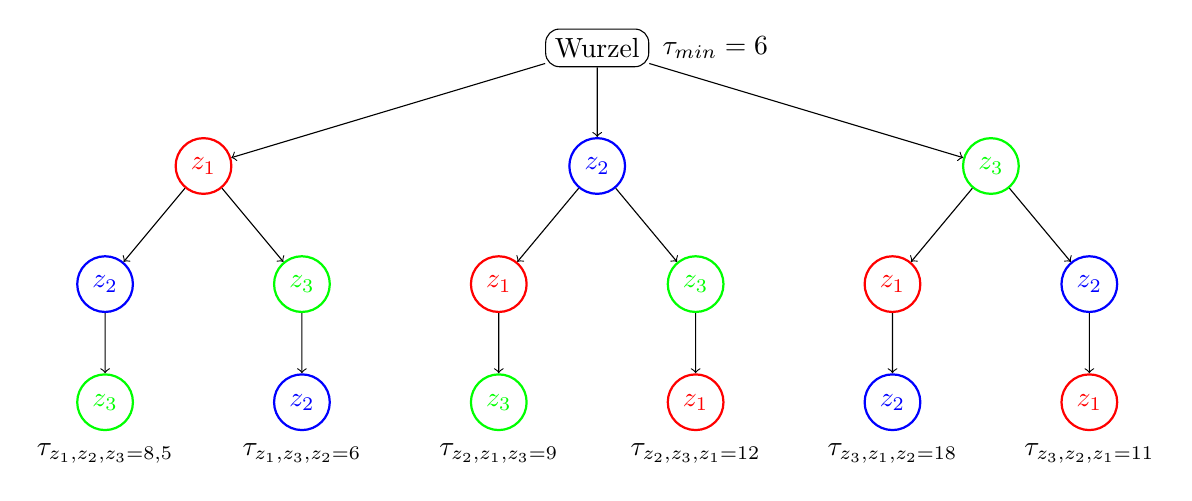
\begin{tikzpicture}[->,level/.style={sibling distance = 5cm/#1,
  level distance = 1.5cm}]
\node[rectangle, draw, rounded corners=5] (root) {\uzlemph{Wurzel}}
	child { node[red]{$z_1$}
		child { node[blue]{$z_2$}
			child { node[green](1){$z_3$} }
		}
		child { node[green]{$z_3$}
			child { node[blue](2){$z_2$} }
		}
	}
	child { node[blue]{$z_2$}
		child { node[red]{$z_1$}
			child { node[green](3){$z_3$} }
		}
		child { node[green]{$z_3$}
			child { node[red](4){$z_1$} }
		}
	}
	child { node[green]{$z_3$}
		child { node[red]{$z_1$}
			child { node[blue](5){$z_2$} }
		}
		child { node[blue]{$z_2$}
			child { node[red](6){$z_1$} }
		}
	};	
\node[above of=root, yshift=-1cm, xshift=1.5cm] {$\tau_{min} = 6$};
\node[below of=1, yshift=0.35cm] {$\tau_{z_1,z_2,z_3 = 8,5}$};
\node[below of=2, yshift=0.35cm] {$\tau_{z_1,z_3,z_2 = 6}$};
\node[below of=3, yshift=0.35cm] {$\tau_{z_2,z_1,z_3 = 9}$};
\node[below of=4, yshift=0.35cm] {$\tau_{z_2,z_3,z_1 = 12}$};
\node[below of=5, yshift=0.35cm] {$\tau_{z_3,z_1,z_2 = 18}$};
\node[below of=6, yshift=0.35cm] {$\tau_{z_3,z_2,z_1 = 11}$};
\end{tikzpicture}
\caption{Die Berechnung der jeweiligen (Teil-)Tourzeit $\tau_{i}, ~1\leq i\leq n!$, für $n!=3!=6$ Permutationen.}
\label{fig:BF1}
\end{figure}

\begin{figure}[htbp]
\centering
\begin{tikzpicture}[->,level/.style={sibling distance = 5cm/#1,
  level distance = 1.5cm}]
\node[rectangle, draw, rounded corners=5] (root) {\uzlemph{Wurzel}}
	child { node[red]{$z_1$}
		child { node[blue]{$z_2$}
			child { node[green]{$z_3$} }
		}
		child { node[green]{$z_3$}
			child { node[blue]{$z_2$} }
		}
	}
	child { node[blue]{$z_2$}
		child { node[red]{$z_1$}
			child { node[green]{$z_3$} }
		}
		child { node[green]{$z_3$}
			child { node[red]{$z_1$} }
		}
	}
	child { node[green](z3){$z_3$}
		child { node[gray]{$z_1$}
			child { node[gray]{$z_2$} }
		}
		child { node[gray]{$z_2$}
			child { node[gray]{$z_1$} }
		}
	};	
\node[above of=root, yshift=-1cm, xshift=1.5cm] {$\tau_{min} = 6$};
\node[below of=1, yshift=0.35cm] {$\tau_{z_1,z_2,z_3 = 8,5}$};
\node[below of=2, yshift=0.35cm] {$\tau_{z_1,z_3,z_2 = 6}$};
\node[below of=3, yshift=0.35cm] {$\tau_{z_2,z_1,z_3 = 9}$};
\node[below of=4, yshift=0.35cm] {$\tau_{z_2,z_3,z_1 = 12}$};
\node[right of=z3, xshift=0.2cm] {$\tau_{z_3} = 6.5$};
\node[red, thick, cross out, below, xshift=4.3cm, yshift=-2.1cm, rotate=50] { };
\node[red, thick, cross out, below, xshift=5.7cm, yshift=-2.1cm, rotate=-50] { };
\end{tikzpicture}
\caption{Mit der Brute-Force-Optimierung wird direkt hinter $z_3$ abgeschnitten, da an diesem Knoten bereits der Zeitpunkt $\tau_{min}$ überschritten wird.}
\label{fig:BF2}
\end{figure}

\scalebox{0.9}{
\begin{minipage}{1\linewidth}
\begin{algorithm}[H]
\begin{algorithmic}
\floatname{algorithm}{Algorithmus}
\caption{Brute-Force-Algorithmus für zwei-orthogonale Achsen beim MT-TSP}
\label{alg:BF}
\State \textbf{Input:} Targets $Z$, pursuer
\State \textbf{Output:} Targets $Z$ Targets Z in order of nondecreasing intercepting time\\

\State Sort $Z$ in order of nonincreasing absolute values of the respective velocities
\State Let $currentTargets$ be the current target order (partial permutation)
\State Let $t$ be the time-array, which represents the intercepting time for each \\
~~~~~target $z_i\in currentTargets$ 
\State $\tau_{min}\leftarrow \infty$
\State $current\leftarrow z_0$
\State $prev\leftarrow origin$, which is determined by the start position of the pursuer\\

\While {there are possible permutations remaining}
\State $current\leftarrow$ the target just intercepted
\State $prev\leftarrow$ the target previously intercepted 
\State $t[current] \leftarrow t[prev] + \pi[prev\rightarrow current]$
\If {$t[current]\geq \tau_{min}$ or at least one target of $Z\backslash currentTargets$ is located\\ ~~~~~~~~between $current$ and $prev$}
\State Step back and follow the next possible permutation-path
\Else
\If {$currentTargets$.length $\neq Z$.length}
\State Choose the next target $z_i$, $z_i\notin currentTargets$
\Else
\State $t[current]\leftarrow t[current] + \pi[current\rightarrow ursprung]$ 
\If {$t[current] < \tau_{min}$}
\State $\tau_{min}\leftarrow t[current]$
\State Step back and follow the next possible permutation-path
\EndIf 
\EndIf
\EndIf
\EndWhile
\end{algorithmic}
\end{algorithm}
\end{minipage}}
\newpage

\subsection{Laufzeitkomplexität Brute-Force-Ansatz}
Betrachten dafür zunächst den Suchbaum ohne die vorgeschlagenen Verbesserungen durch Beschneidungen. Der Suchbaum besitzt dabei $V_n = n + n\cdot (V_{n-1})$ Knoten, wodurch die Berechnung des kompletten Baums mit $\mathcal{O}(n!)$ abgeschätzt werden kann. 
Diese Laufzeit gilt allerdings nur für $n\leq 4$, solange die Ziele verteilt auf den Seiten \emph{Left, Right, Top} und \emph{Bottom} liegen. Für größere Eingaben liegen definitiv Ziele zwischen anderen Zielen, wodurch mit dem 2. Szenario der Baum beschnitten wird. 

Für $n>4$ ist die Anzahl der Beschneidungen sehr schwer vorherzusagen. Dies hängt stark von der Eingabegröße ab. Generell konvergiert das Verhältnis von betrachteten Knoten zu $V_n$ gegen $\delta$, wobei $\delta>0$ und $n>12$ (mehr dazu im Kapitel \ref{kap5:bf}). Eine Approximation würde dabei einen Faktor für die Laufzeit bestimmen, welcher in der Komplexität allerdings vernachlässigt werden kann. Somit hat der Brute-Force-Algorithmus trotzdem eine Zeitkomplexität von $\mathcal{O}(n!)$.

\subsection{Korrektheit Brute-Force-Ansatz}
Mit dem Brute-Force-Algorithmus wird jede mögliche Permutation an Zielen ausprobiert. Bei der Berechnung einer Permutation werden alle Ziele nacheinander abgefangen und der Zeitstempel mit der Zeit erhöht, die zum Abfangen des jeweiligen Ziels benötigt wird. Sofern eine Permutation schneller als die aktuell schnellste ist, wird diese übernommen und $\tau_{min}$ mit der benötigten Tourzeit überschrieben. Mit den Verbesserungen wird der Permutationsbaum beschnitten und es werden Berechnungen eingespart. Somit wird garantiert, dass die optimale Tour zurückgegeben wird.


\chapter{Experimente}
\label{kap5}
In diesem Kapitel werden die drei Algorithmen
\begin{itemize}
\item 1D-Algorithmus
\item Prioritäts-Algorithmus
\item Brute-Force-Algorithmus
\end{itemize}
mit verschiedenen Instanzen getestet. Beim 1D-Algorithmus reicht es, diesen auf spezielle Eingaben zu testen. Anschließend wird beim Brute-Force-Algorithmus mit unterschiedlichen Eingabegrößen auf die Abschneidungen und die damit resultierenden Einsparungen bei der Berechnung der Permutationen getestet. Danach wird der Prioritäts-Algorithmus gegen den BF-Algorithmus laufen gelassen, um die dadurch resultierende Güte zu bestimmen. Zuletzt wird der Prioritäts-Algorithmus mit verschiedenen Kombinationen an Parametern betrachtet. 

\section{Durchschnittliche Laufzeit des 1D-Algorithmus}

Der eindimensionale Algorithmus (siehe Algorithmus \ref{alg:1D}) findet optimale Lösungen innerhalb von $\mathcal{O}(n^2)$. Dabei ist interessant, wie sich die Laufzeit bei verschiedenen Instanzen verhält. Es werden im Folgenden Eingaben von bis zu $1000$ Zielen getestet. Dabei wird die Verfolgergeschwindigkeit auf $v_\kappa=40$ festgesetzt, wodurch sich jedes Ziel $z_i$ mit $|v_i|<v_\kappa$ fortbewegt. Außerdem sind die Startkoordinaten der Ziele zwischen $-10.000$ und $10.000$ limitiert. Dies ist gerade bei $n=1.000$ nötig, da die Ziele direkt nebeneinander starten. Mit diesen Bedingungen wird jedes der $n$ Ziele die Geschwindigkeit und Startposition für einen Testdurchlauf zufällig generiert. Für jede der Eingabegrößen wird für $100$ Instanzen jeweils die Laufzeit getestet. Anschließend wird der Durchschnitt bestimmt. 

Die Ergebnisse in Abbildung \ref{fig:Exp1D} zeigen einen nahezu konstanten Anstieg der durchschnittlichen Laufzeit. Untersucht man die einzelnen Ausgaben der zufälligen Instanzen, wird der Zusammenhang schnell klar. Durch die Eliminierungen werden in nahezu allen Fällen die meisten Ziele aus $Left$ und $Right$ entfernt. Mit dem $Preprocessing$- und dem $Postprocessing$-Schritt werden sind weiterhin quadratische Laufzeiten nötig. Die eigentliche Berechnung der optimalen Tour über die Zustände ist dann äquivalent zu deutlich kleineren Instanzen. Somit wächst die durchschnittliche Laufzeit nahezu lineare an. 

\newpage
\begin{figure}[htpb]
\centering
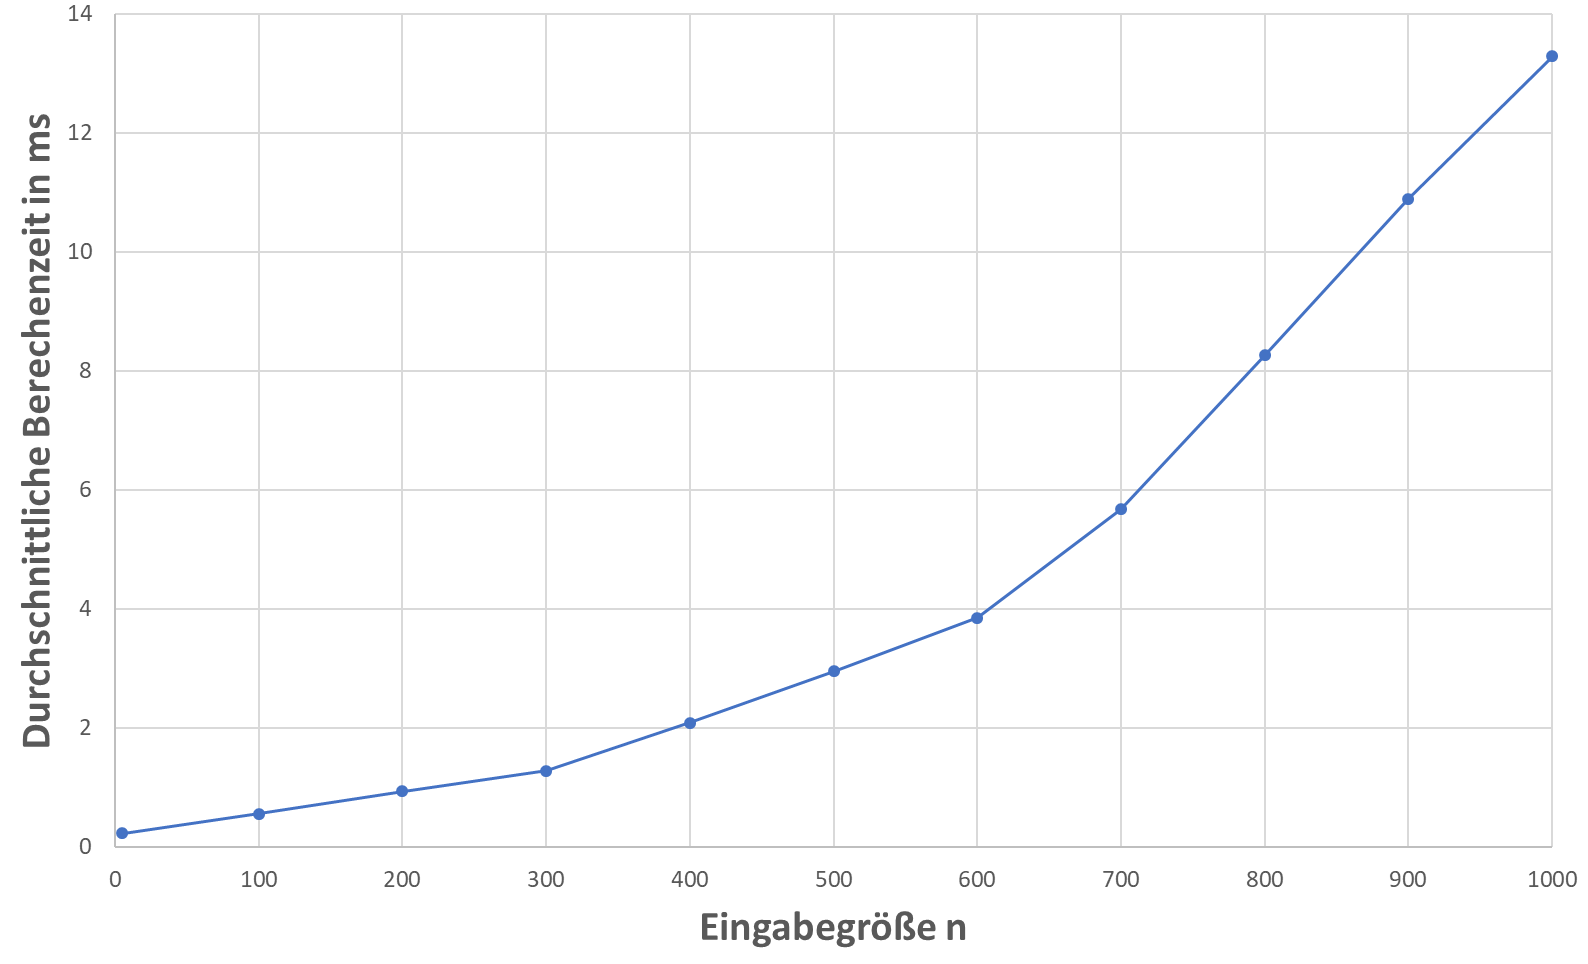
\includegraphics[scale=0.24]{../Grafiken/Verwendete/Exp1D_2.png}
\caption{Nahezu konstanter Anstieg der durchschnittlichen Berechenzeit von $100$ Instanzen bei steigender Eingabegröße.}
\label{fig:Exp1D}
\end{figure} 
\newpage

\section{Brute-Force-Algorithmus mit unterschiedlichen Eingabegrößen}
\label{kap5:bf}

Gängige Brute-Force-Ansätze sind bei Eingabegrößen mit Zielen sehr ineffizient. Bereits bei $n=10$ ist mit $n!=3.628.800$ möglichen Permutationen eine Berechnung sehr aufwendig. Mit den vorgeschlagenen Beschneidungen des Suchbaums soll dem Abhilfe geschaffen werden. Dies wird nachfolgend analysiert. Hierfür wurde der Brute-Force-Algorithmus für $n\in\{1,\dots,14\}$ getestet (siehe Tabelle \ref{tab:ExpBF}). Dabei wird die Verfolgergeschwindigkeit mit $v_{\kappa}=40$ festgesetzt. Zudem startet jedes Ziel bei einer Koordinate zwischen $-100$ und $100$ auf einer der Achsen. Damit wird jeweils für ein Ziel die Geschwindigkeit und Startposition für einen Testdurchlauf zufällig generiert.

Je größer die Anzahl an \emph{Instanzen}, desto repräsentativer sind die Ergebnisse des Datensatzes für die jeweilige Eingabegröße. Für die nachfolgenden Attribute wird für der Durchschnitt aus allen Instanzen berechnet. Die in dem Suchbaum \emph{betrachteten Knoten} geben an, wie viele Ziele insgesamt berechnet wurden. Somit kann mit \emph{Anteil Knoten} durch die Berechnung des Verhältnisses von den \emph{betrachteten Knoten} und $V_n$ abgewogen werden, wie viele Knoten des Baums berechnet wurde. Je niedriger dieser Wert, desto mehr wurde im Baum abgeschnitten. Mit dem $Schnitte$-Attribut kann die Anzahl an Beschneidungen im Baum bestimmt werden. Dieser Wert ist allerdings nur in Kombination mit den \emph{betrachteten Knoten} repräsentativ, da die Schnitte an jeder Stelle im Baum möglich sind\footnote{Ein Schnitt in der Nähe der Wurzel sorgt für eine starke Reduzierung an betrachteten Knoten, während ein Schnitt weit unten genau das Gegenteil bewirkt.}. Sobald eine Instanz aufgrund eines \emph{Heap-Space}-Fehlers\footnote{Die Algorithmen dieser Arbeit sind jeweils in Java über programmiert. Um dies zu umgehen sind leistungsstärkere Rechner notwendig.} nicht berechnet werden kann, wird dies in \emph{Fails} festgehalten.
 
Bei zunehmender Eingabegröße steigt die Anzahl an betrachteten Knoten mit dem Faktor $\approx 4$ nahezu konstant an. Im Gegenzug sinkt zusätzlich der Anteil der Knoten und die Anzahl an Schnitten nimmt zu. Auch die Anzahl der Blätter bzw. Permutationen steigen nur langsam an. Dies zeigt, dass bei ansteigender Eingabegröße, die Komplexität der Berechnung gar nicht so stark ansteigt. Bei $n=13$ werden im Schnitt gerade einmal $4.303,92$ von möglichen $6.227.020.800$ Blättern ausgerechnet. Damit konvergiert der Anteil an betrachteten Knoten gegenüber der Gesamtknotenanzahl bereits ab wenig Zielen gegen $0$. Man würde nun annehmen, dass der Brute-Force-Algorithmus auch für größere $n$ eine gute Ergebnisse liefert. Allerdings erkennt man schon ab $n=10$, dass die Berechnungen immer länger dauern und sehr viele Ressourcen beziehen. Bei $n=14$ ereignen sich die ersten Fehler, wodurch nur noch $3$ Berechnungen durchgeführt werden. Die langen Berechnungszeiten sind auf Fälle zurückzuführen, in denen nicht nach kurzer Zeit ein kleines $\tau_{min}$ gefunden wurde. Damit werden bei steigender Eingabegröße erheblich mehr Berechnungen durchgeführt, da der eigentliche Suchbaum ohne Beschneidungen eine Größe von $n!$ Permutationen besitzt.  

Die Ergebnisse fallen für diese Laufzeit trotzdem sehr positiv aus, da normale Brute-Force-Heuristiken bereits bei $n>10$ sehr langsam laufen und bei einer guten Vorsortierung potentiell auch Fälle mit $n=15$ durch große Abschneidungen in der Nähe der Wurzel lösbar sind. Die in diesem Fall verwendete Sortierung nach dem Betrag der Geschwindigkeit ist sehr simpel und zeigt, dass eine etwas komplexere Sortierung\footnote{Es könnten auch hier zusätzlich Prioritäten verwendet werden.} sehr wahrscheinlich schneller ein kleines $\tau_{min}$ finden kann. 

Ab einer Eingabegröße von $n>12$ ereignen sich \emph{Heap-Space}-Fehler. Dies liegt daran, dass sehr viele Knoten betrachtet werden, aber nicht genug Rechenkapazität zur Verfügung stand. Mit einer anderen Programmiersprache oder einem leistungsstärkeren Rechner könnte man vermutlich $n=13$ fehlerfrei berechnen. Durch die Fehler ist der Datensatz mit $n=14$ nicht mehr repräsentativ, da hierbei nur drei Instanzen berechnet werden konnten. Dabei wurde bei der ersten Instanz sehr früh ein kleines $\tau_{min}$ gefunden, wodurch der Schnitt der jeweiligen Attribute sehr niedrig ist.   \\~\\

\begin{table}[htpb]
\centering
\scalebox{0.93}{
\begin{tabular}{ccccccc} 
\uzlhline
\uzlemph{$n$} &\uzlemph{Instanzen}&\uzlemph{$\diameter$betr. Knoten} & \uzlemph{$\diameter$Anteil Knoten} & \uzlemph{$\diameter$Schnitte} & \uzlemph{$\diameter$ber. Blätter} & \uzlemph{Fails}\\ \uzlhline
1& 10.000& ~~~~~~~~~~~1,00& 1,000000& ~~~~~~~~0,00& ~~~~1,00& ~0 \\
2& 10.000& ~~~~~~~~~~~3,75& 0,939151& ~~~~~~~~0,24& ~~~~1,57& ~0 \\
3& 10.000& ~~~~~~~~~~11,75& 0,783513& ~~~~~~~~0,95& ~~~~3,14& ~0 \\
4& 10.000& ~~~~~~~~~~37,81& 0,590758& ~~~~~~~~3,22& ~~~~6,71& ~0 \\
5& 10.000& ~~~~~~~~~130,44& 0,401344& ~~~~~~~11,87& ~~~15,02& ~0 \\
6& 10.000& ~~~~~~~~~471,76& 0,241184& ~~~~~~~47,23& ~~~32,46& ~0 \\
7& 10.000& ~~~~~1.819,94& 0,132852& ~~~~~~194,96& ~~~70,33& ~0 \\
8& 10.000& ~~~~~7.353,01& 0,067090& ~~~~~~852,13& ~~150,30& ~0 \\
9& 10.000& ~~~~31.426,98& 0,031860& ~~~~3.833,61& ~~313,76& ~0 \\
10&~1.000& ~~~140.342,54& 0,014228& ~~~18.169,79& ~~620,86& ~0 \\
11&~1.000& ~~~650.570,40& 0,005996& ~~~88.862,13& 1.304,56& ~0 \\
12&~~~100& 3.562.601,51& 0,002736& ~~457.589,77& 3.246,11& ~0 \\
13&~~~100& 8.184.931,87& 0,000484& 1.523.396,29& 4.303,92& 22\\
14&~~~~10& 5.033.246,67& 0,000021& 1.147.070,33& 2.025,67& ~7 \\ \uzlhline
\end{tabular}}
\caption{Beschneidungen im Suchbaum des Brute-Force-Algorithmus bei einer Eingabe von $1\leq n\leq 14$ Zielen}
\label{tab:ExpBF}
\end{table}
\newpage

\section{Wahl der Gewichte für den Prioritäts-Algorithmus}
\label{kap5:gewichte}

Offensichtlich gibt es keine universellen Gewichte, die gute Ergebnisse garantieren. In diesem Abschnitt sollen trotzdem Gewichte präsentiert, die für zufällige Instanzen gute Ergebnisse ermöglichen. Hierfür wird die Verfolgergeschwindigkeit auf $v_{\kappa}=40$ gesetzt. Im Folgenden  werden für die Eingabegrößen $n\in\{8,10,12\}$ und den Betrag der Startkoordinatenlimits $[100,10.000]$ jegliche Kombinationen getestet. Für jedes der Ziele werden mit diesen Bedingungen die Geschwindigkeit und Startposition für einen Testdurchlauf zufällig generiert.

Die Gewichte aus Tabelle \ref{tab:ExpGewichte} belegen, wie auch schon erwähnt, dass es keine universellen Gewichte gibt. Allerdings wird mit der Tabelle ein grobes Verhältnis der Gewichte deutlich. Dabei ist $w_1$ mindestens doppelt so groß wie $w_2$. Das Gewicht $w_3$ variiert hingegen im Verhältnis zu $w_1$ stärker und ist für einige Instanzen zum Teil größer als $w_1$. Allerdings gibt es auch Instanzen, in denen $w_2$ als größtes Gewicht die besten Ergebnisse erzielt. Im Folgenden werden die Gewichte $\omega = \{87,34,31\}$ gewählt. Diese Gewichte haben sich für eine große Menge an Testinstanzen bewährt und werden somit auch für die nachfolgenden Experimente gewählt. \\~\\

\begin{table}[htpb]
\centering
\scalebox{1}{
\begin{tabular}{cccc} 
\uzlhline
$n$ & |Koordinatenlimit| & $\omega$\\ \uzlhline
~8& ~~~~100& $\{64,21,19\}$ \\
~8&  10.000& $\{54,17,40\}$ \\
10& ~~~~100& $\{98,39,74\}$ \\
10&  10.000& ~~~~$\{75,3,6\}$ \\
12& ~~~~100& ~~$\{69,14,8\}$ \\
12&  10.000& ~~~~$\{24,4,7\}$ \\
\uzlhline
\end{tabular}}
\caption{Der jeweils beste Gewichte-Kandidat von $1.000$ zufälligen Gewichten für $100$ zufällige Instanzen.}
\label{tab:ExpGewichte}
\end{table} 
\newpage

\section{Güte des Prioritäts-Algorithmus}
Der Prioritäts-Algorithmus gilt mit einer Laufzeit von $\mathcal{O}(n^2)$ als sehr effizient. Da dieser keine optimalen Touren garantiert, muss nun abgeschätzt werden, ob die Ergebnisse zufriedenstellend sind. Dafür lassen wir den Algorithmus gegen den Brute-Force-\\Algorithmus laufen, um die Güte zu bestimmen. Der Prioritäts-Algorithmus erzeugt bei einer Instanz $I$ eine Ausgabe der Laufzeit mit $prio(I)$. Die Güte $r_I$ wird für eine Instanz mit
\begin{align*}
r_I = \dfrac{prio(I)}{opt(I)}
\end{align*} 
berechnet, wobei für $opt(I)$ der Brute-Force-Algorithmus verwendet werden kann, da eine optimale Lösung garantiert wird. Der Brute-Force-Algorithmus läuft bis $n=12$ einigermaßen schnell und wird demnach als größte Testeingabe gewählt. Es wird nun für jede mögliche Kombination aus den folgenden Parametern
\begin{align*}
n&\in\{8,10,12\}\\
max\{v_{i}\}\footnotemark&\in\{20,40,60\} 
\end{align*}
\footnotetext{Dies bezeichnet die Maximalgeschwindigkeit eines jeden Ziels $z_i\in Z$}
 betrachtet und mit bis zu $10.000$ Instanzen getestet\footnote{Die Laufzeit steigt mit der Eingabegröße stark an, demnach wird für $n=10$ und $n=12$ eine Instanzenanzahl von $1.000$ bzw. $100$ getestet.}. Mit den Instanzen wird jeweils die \emph{maximale} und \emph{durchschnittliche Güte} des Prioritäts-Algorithmus berechnet Zudem wird die Anzahl an \emph{optimalen Touren} und deren \emph{Anteil} an den Instanzen berechnet. Die Verfolgergeschwindigkeit $v_{\kappa}=61$ und die Startkoordinaten der Ziele zwischen $-100$ und $100$ werden als feste Parameter gewählt. Als Gewichte für die Berechnung der Priorität wird $\omega = \{87,34,31\}$ verwendet. Die Ergebnisse werden in Tabelle \ref{tab:ExpGüte} präsentiert.

Dies sind sehr überraschende Ergebnisse, da hierbei viele Erkenntnisse gewonnen werden. Zunächst fällt für $max\{v_i\}=60$ jeweils eine gravierende maximale Güte auf. Das hängt damit zusammen, dass der Algorithmus nur aktuelle Ziele betrachtet und in diesem Schritt keine Berechnung für potentiell folgende Ziele getätigt wird. Bei der Durchführung ist aufgefallen, dass diese worst-case-Szenarien vor allem auftreten, wenn mehrere Zielen eine Geschwindigkeit von $v_i=60$ besitzen. Um dafür eine optimale Lösung zu garantieren, müssten auf die Instanz abgestimmte Gewichte $\omega$ gewählt werden. Durch diese Ausnahmefälle steigt auch die durchschnittliche Güte stark an. 

Bei steigender Eingabegröße verringern sich der Anteil der optimalen Touren quasi konstant. Das lässt vermuten, dass ab $n=14$ quasi keine optimalen Lösungen mehr gefunden werden. Mit dieser Überlegung wäre der Prioritäts-Algorithmus keine gute Option ab $n>10$, da kaum noch optimale Lösungen gefunden werden. Betrachtet man allerdings nun die durchschnittliche Güte, ist der Algorithmus vielleicht doch für große Eingabegrößen geeignet. Diese ist nahezu konstant für alle die jeweiligen maximalen Geschwindigkeiten der Ziele. Mit der konstanten durchschnittlichen Güte werden somit trotz sinkender Anzahl an optimalen Touren weiterhin schnelle Touren berechnet. Für solche Eingabegrößen ist dies allerdings nur spekulativ, da ab $n>12$ mit dem Brute-Force-Algorithmus die Güte nicht mehr präzise genug ausgerechnet werden kann. Im Endeffekt steht und fällt der Algorithmus mit den gewählten Gewichten. \\~\\

\begin{table}[htpb]
\centering
\scalebox{1}{
\begin{tabular}{ccccccc} 
\uzlhline
\uzlemph{$n$} & \uzlemph{Instanzen}& \uzlemph{$max\{v_i\}$} & \uzlemph{$\diameter$Güte} & \uzlemph{max Güte} & \uzlemph{opt. Touren} & \uzlemph{Anteil opt.}\\ \uzlhline
~8& 10.000& 20& 1,10& ~~2,59& 6313& 0,63 \\
~8& 10.000& 40& 1,41& ~11,93& 3341& 0,33 \\
~8& 10.000& 60& 3,53& 328,88& 1390& 0,14 \\
10& ~~1.000& 20& 1,14& ~~2,15& ~518& 0,52 \\
10& ~~1.000& 40& 1,54& ~~9,22& ~220& 0,22 \\
10& ~~1.000& 60& 5,32& 282,26& ~~83& 0,08 \\
12& ~~~~~~100& 20& 1,16& ~~2,31& ~~43& 0,43 \\
12& ~~~~~~100& 40& 1,56& ~~4,79& ~~12& 0,12 \\
12& ~~~~~~100& 60& 5,30& ~82,29& ~~~5& 0,05 \\ \uzlhline
\end{tabular}}
\caption{Güte des Prioritäts-Algorithmus}
\label{tab:ExpGüte}
\end{table}
\newpage

\section{Große Eingaben für den Prioritäts-Algorithmus}
Es wird nun das Verhalten des Prioritäts-Algorithmus für Instanzen mit vielen Zielen getestet. Dabei kann keine Korrektheit mehr bewiesen werden, da der Brute-Force-\\Algorithmus für solche Eingabegrößen nicht geeignet ist. Die Startkoordinaten der Ziele werden dabei zwischen $-250$ und $250$ zufällig gewählt. Die Eingabegröße liegt für dieses Experiment zwischen $5$ und $100$. Die Geschwindigkeit wird in drei verschiedenen Kombinationen von Zielen und Verfolger getestet:
\begin{itemize}
\item $20-200$: langsame Ziele, schneller Verfolger
\item $40-100$: Differenz der Geschwindigkeiten verringert sich etwas
\item $60-~~~61$:~Verfolger ist nur minimal schneller
\end{itemize}
Diese Wahl der Startkoordinaten und Geschwindigkeiten wurden aus \cite{stieber2015multiple} übernommen. Bemerke, dass es sich bei den Geschwindigkeiten der Ziele im Gegenzug zu vorherigen Tests nicht um Maximalgeschwindigkeiten handelt, sondern festgesetzt sind. Da allerdings nur ein Verfolger betrachtet wird, kann $v_{\kappa}$ um einen Wert inkrementiert werden. Somit werden unendliche Tourzeiten verhindert. Auch in diesem Experiment werden die Gewichte $\omega = \{87,34,31\}$ verwendet. In Tabelle \ref{tab:ExpPrio} sind die Ergebnisse aus den verschiedenen Kombinationen präsentiert.

Mit den vorherigen Ergebnissen von Tabelle \ref{tab:ExpGüte} wird nun klar, dass die Änderungen der Geschwindigkeiten der Ziele beim Prioritäts-Algorithmus die Tourzeiten stark beeinflussen. Es kann nun grundsätzlich gesagt werden, dass der Algorithmus sehr effizient ist, sobald der Verfolger deutlich schneller ist, als jedes gegebene Ziel. Für sehr gute Ergebnisse ist in diesem Fall also eine Differenz der Geschwindigkeiten von mindestens $40$ zu empfehlen. Für Instanzen mit sehr kleinen Differenzen sind die berechneten Touren ggf. weit entfernt von einer optimalen Lösung. \\

\begin{table}[htpb]
\centering
\scalebox{1}{
\begin{tabular}{cccc} 
\uzlhline
\uzlemph{$n$} & \uzlemph{$v_i$}& \uzlemph{$v_{\kappa}$} & \uzlemph{Tourzeit} \\ \uzlhline
~~~~5& 20 & 200 & ~~~~~~~~~~~~~~~~~4.11 \\
~~~~5& 40 & 100 & ~~~~~~~~~~~~~~~15.59 \\
~~~~5& 60 & ~~61 & ~~~~~~7.198.012 \\
~~25& 20 & 200 & ~~~~~~~~~~~~~~~12.75 \\
~~25& 40 & 100 & ~~~~~~~~~~~~~~136.28 \\
~~25& 60 & ~~61 & 1.199.646.497 \\
~~50& 20 & 200 & ~~~~~~~~~~~~~~~13.46 \\
~~50& 40 & 100 & ~~~~~~~~~~~~~~149.14 \\
~~50& 60 & ~~61 & 1.622.776.018 \\
~~75& 20 & 200 & ~~~~~~~~~~~~~~~17.28 \\
~~75& 40 & 100 & ~~~~~~~~~~~~~~168.81 \\
~~75& 60 & ~~61 & 1.747.321.268 \\
100& 20 & 200 & ~~~~~~~~~~~~~~~14.17 \\
100& 40 & 100 & ~~~~~~~~~~~~~~164.75 \\
100& 60 & ~~61 & 1.615.929.568 \\
\uzlhline
\end{tabular}}
\caption{Ziele mit gleichen Geschwindigkeiten im Prioritäts-Algorithmus}
\label{tab:ExpPrio}
\end{table}

%\chapter{Conclusion}
\chapter{Zusammenfassung und Ausblick}
%-------------------Ergebnisse der Arbeit--------------------
Die Lemmata aus Kapitel \ref{kap4} zeigen, dass für optimale Touren dieselben Eigenschaften von eindimensionalen MT-TSP auch für zwei-orthogonale-Achsen im MT-TSP gelten. Im Kapitel \ref{kap5} wurde gezeigt, dass der Algorithmus für eindimensionale MT-TSP von \cite{helvig} auch bei großen Instanzen eine starke Performance aufweist, da im Vorwege viele Ziele eliminiert werden können. 
Der Prioritäts-Algorithmus ist sehr abhängig von den gewählten Gewichten. Dabei haben sich für generelle Fälle die Gewichte $\omega=\{87,34,31\}$ etabliert. Sobald der Verfolger um $40$ Geschwindigkeit-Einheiten schneller ist, als das schnellste Ziel der Instanz, werden gute bis optimale Touren von dem Algorithmus nahezu garantiert. Die Güte bleibt bei steigender Eingabegröße nahezu gleich. Der Brute-Force-Algorithmus liefert für kleine Instanzen sehr effizient optimale Ergebnisse. Dabei konvergieren das Verhältnis der betrachteten Knoten zu den Gesamtknoten durch große Abschneidungen im Baum gegen $0$, wodurch im Gegensatz zu herkömmlichen Brute-Force-Heuristiken auch Instanzen mit $n=14$ ggf. schnell berechnet werden können. 

%----------------------Verbesserungen------------------------
Zwar wurden die Probleme bei der Modellierung als Graphen aufgezeigt, ausgeschlossen sei diese allerdings nicht. Mit dem Ansatz über das Lemma \ref{lem:2} sollte eine optimale Strategie definitiv möglich sein und welche eine geringere Laufzeit aufweist, als der Brute-Force-Algorithmus. Der Brute-Force-Ansatz kann über die vorgeschlagenen \\Beschneidungs-Szenarien um einiges verbessert werden. Dafür kann in jedem Knoten eine Sortierung der Nachfolgeknoten durchgeführt werden. Zudem können Ziele im eliminiert werden, welche so oder so von dem Verfolger abgefangen werden. Diese werden dann, wie im  Algorithmus \ref{alg:1D}, im Nachhinein wieder hinzugefügt. Dennoch können lange Laufzeiten bei worst-case-Szenarien nicht ausgeschlossen werden, weshalb der Brute-Force-Algorithmus bei großen Instanzen weiterhin  untauglich ist. Beim Prioritäts-\\Algorithmus könnten zudem im Vorwege Ziele eliminiert werden, welche sowieso eingeholt und damit im Algorithmus gar nicht erst betrachtet werden. 

%-------------------------Ausblick---------------------------
Mit dem Prioritäts-Algorithmus wurde zum Einen ein effizienter und mit dem Brute-Force-Ansatz zum Anderen ein optimaler Algorithmus für wenig Ziele vorgestellt. Für zukünftige Arbeit wäre ein einigermaßen effizienter, aber optimaler Algorithmus vom großen Interesse. Dies wäre ein notwendiger Schritt, um theoretische Arbeit für $k$-Achsen in MT-TSP zu leisten. Die dazu gewonnenen theoretischen Resultate aus Kapitel \ref{kap3} waren zwar nützlich, einen exakten Algorithmus für große Eingaben konnte aus zeitlichen Gründen aber nicht präsentiert werden. Darüber hinaus ist das nächste Ziel in dieser Thematik die Betrachtung von zweidimensionalen MT-TSP und das Aufstellen von Heuristiken. Diesen Jahres wurde für generelle Fälle eine Arbeit \cite{moraes} veröffentlicht, in der mit evolutionären Strategien versucht wird, auf eine optimale Tour in vielen Iterationen hinzuarbeiten. Dabei ist allerdings die optimale Tour von vielen verschiedenen Parametern abhängig und garantieren keine optimale Lösung. 



\begin{bibtex-entries}
@article{helvig,
  title={The moving-target traveling salesman problem},
  author={Helvig, Christopher S and Robins, Gabriel and Zelikovsky, Alex},
  journal={Journal of Algorithms},
  volume={49},
  number={1},
  pages={153--174},
  year={2003},
  publisher={Elsevier}
}

@article{moraes,
  title={Experimental Analysis of Heuristic Solutions for the Moving Target Traveling Salesman Problem Applied to a Moving Targets Monitoring System},
  author={de Moraes, Rodrigo S and de Freitas, Edison P},
  journal={Expert Systems with Applications},
  volume={136},
  pages={392--409},
  year={2019},
  publisher={Elsevier}
}

@inproceedings{hammar,
  title={Approximation results for kinetic variants of TSP},
  author={Hammar, Mikael and Nilsson, Bengt J},
  booktitle={International Colloquium on Automata, Languages, and Programming},
  pages={392--401},
  year={1999},
  organization={Springer}
}

@incollection{brandstadt1994kurzeste,
  title={K{\"u}rzeste Wege},
  author={Brandst{\"a}dt, Andreas},
  booktitle={Graphen und Algorithmen},
  pages={106--123},
  year={1994},
  publisher={Springer}
}

@article{kaaser2014algorithmen,
  title={Algorithmen und Datenstrukturen},
  author={Kaaser, Dominik S},
  year={2014}
}

@book{kunzi2013einfuhrungskursus,
  title={Einf{\"u}hrungskursus in die dynamische Programmierung},
  author={K{\"u}nzi, Hans Paul and Nievergelt, Erwin},
  volume={6},
  year={2013},
  publisher={Springer-Verlag}
}

@article{choubey2013moving,
  title={Moving target travelling salesman problem using genetic algorithm},
  author={Choubey, Nitin S},
  journal={International Journal of Computer Applications},
  volume={70},
  number={2},
  year={2013},
  publisher={Foundation of Computer Science}
}

@book{weicker2015evolutionare,
  title={Evolution{\"a}re algorithmen},
  author={Weicker, Karsten},
  pages={24--25},
  year={2015},
  publisher={Springer-Verlag}
}
  
@book{minx2015autonomes,
  title={Autonomes Fahren},
  author={Minx, Eckard and Dietrich, Rainer},
  year={2015},
  publisher={Piper ebooks}
}

@article{stieber2015multiple,
  title={The multiple traveling salesmen problem with moving targets},
  author={Stieber, Anke and F{\"u}genschuh, Armin and Epp, Maria and Knapp, Matthias and Rothe, Hendrik},
  journal={Optimization Letters},
  volume={9},
  number={8},
  pages={1569--1583},
  year={2015},
  publisher={Springer}
}

\end{bibtex-entries}

% If you need to have an appendix (I advise against it), insert it
% here using, first, \appendix and then \chapter and then,
% possibly, \section. 
%
\appendix
\chapter{Implementierungen}

Bei den beigefügten Java-Klassen handelt es sich um die Implementation folgender in dieser Arbeit vorgestellten Algorithmen:
\begin{itemize}
\item 1D-Algorithmus
\item Prioritäts-Algorithmus
\item Brute-Force-Algorithmus
\end{itemize} 
Diese habe ich anhand der Pseudocodes Algorithmus \ref{alg:1D}, Algorithmus \ref{alg:2OA.1} und Algorithmus \ref{alg:BF} implementiert. Der Quellcode umfasst insgesamt ca. 2300 Zeilen, inklusive einiger Testmethoden, welche für Kapitel \ref{kap5} verwendet wurden. Nachfolgend wird beschrieben, wie die zugehörigen Klassen verwendet werden und zu verstehen sind. 

\section{Funktionsweise des Programmes und Relationen zwischen den Klassen}
Die Klasse \emph{Constants.java} besitzt alle nötigen Parameter für die Algorithmen und Testmethoden, welche in Tabelle \ref{Constants} abgebildet werden. Es kann mit Hilfe der Parameter ein zufälliger Input mit \emph{GenerateInput.java} generiert oder ein bestimmter Input vorgegeben werden. Der Input besitzt dabei die Form ``1D\_<x>.txt''- oder ``2OA\_<x>.txt''-Datei, je nachdem, ob ein 1D-Fall oder zwei-orthogonale-Achsen-Fall betrachtet wird. Die \emph{main}-Methode liegt in \emph{Main.java}. Diese berechnet abhängig von den Konstanten einen der beiden Fälle oder startet eine der Test-Methoden. 

Die Berechnung der 1D-Fälle erfolgt mit der Klasse \emph{SolveOneDim.java}, bei zwei-\\orthogonale-Achsen-Fälle wird die Tour mit \emph{SolveWithPriorityApproach} oder \emph{SolveWithBruteForce} berechnet. Die drei Klassen wandeln jeweils den Input in eine Liste von \emph{Target.java}-Objekten um. \emph{SolveOneDim.java} verwendet zusätzlich für die Zustandsliste die Klasse \emph{State.java}. Der Suchbaum des Brute-Force-Algorithmus wird mit \emph{SequenceStep} berechnet, indem für Kinderknoten neue \emph{SequenceStep}-Objekte erstellt werden. In jedem Schritt wird dann auf eine Abschneidung überprüft. 

Mit \emph{CalcSequence} kann eine exakte Zeit bestimmt werden, die eine bestimmte Reihenfolge an Zielen benötigt. Dabei wird nicht auf Ziele überprüft, welche auf dem Weg zu dem nächsten Ziel abgefangen wurden. Es kann also eine Tour eines der Algorithmen in der Reihenfolge der Tour in ``Seq.txt'' gespeichert werden, welche anschließend berechnet wird. Damit kann sichergestellt werden, dass die Tour korrekt berechnet wurde. Dies ist bei Randbedingungen sinnvoll und fördert zugleich das Debuggen. 

\section{Testumgebung für die Experimente}

Die Testumgebung befindet sich innerhalb der $Main.java$. Ab dem Parameter \\\emph{TESTING\_ENABLED} aus Tabelle \ref{Constants} werden anstelle der normalen Berechnungen die Testmethoden in \emph{Main.java} verwendet. Für 1D-Fälle wird dabei die Laufzeit für zufällige Instanzen in \emph{test1DRuntime} getestet. 

Bei zwei-ortogonale-Achsen-Fällen werden verschiedene Tests durchgeführt. Mit \emph{testPrioWithMultipleInstances} werden zufällige Gewichte für zufällig generierte Instanzen\\ durchprobiert und am Ende die besten $10$ Gewichte-Tripel in eine Datei geschrieben. Der Suchbaum beim Brute-Force-Algorithmus wird in \emph{testBFWithMultipleInstances} ebenfalls für zufällige Instanzen analysiert und die Ergebnisse in einer Datei festgehalten. Mit \emph{testPrioQuality} wird die Güte des Prioritäts-Algorithmus für zufällige Instanzen berechnet und weitere Ergebnisse, wie die maximale Güte, in eine Datei geschrieben. Es kann aber auch nur eine Instanz getestet werden. Für diese werden in \emph{testWeightsWithBruteForce} Gewichte zufällig generiert und bei optimalen Ergebnisse werden die Gewichten in eine andere Datei festgehalten. In \emph{testWeightsWithoutBruteForce} werden die Gewichte, zufällig gewählt, festgehalten, die bessere Ergebnisse erzielen, als jene in der vorherigen Iteration. Für \emph{testWeightsWithBruteForce} und \emph{testWeightsWithoutBruteForce} kann mit \emph{calcWeightAverage} der Durchschnitt der Gewichte berechnet werden.

\begin{table}[htpb]
\centering
\footnotesize
\scalebox{0.9}{
\begin{tabular}{lll} \uzlhline
\uzlemph{Parameter} & \uzlemph{Datentyp} & \uzlemph{Bedeutung/Belegung} \\ \uzlhline
&& Welcher Fall/Instanz soll berechnet werden? \\
IS\_1D & boolean                          & true: 1D-Fall \\ 
&& false: 2OA-Fall \\\uzlhline
&& Soll eine zufällige Eingabe generiert werden?\\
GENERATE\_NEW\_INPUT & boolean            & true: Ja \\ 
&& false: Eigene Eingabe-Datei verwenden \\\uzlhline
INPUT\_FILE\_1D & String                  & 1D-Instanz-Datei \\ \uzlhline
INPUT\_FILE\_2OA & String                 & 2OA-Instanz-Datei \\ \uzlhline
USE\_BRUTE\_FORCE & boolean               & Brute-Force-Algorithmus verwenden? \footnotemark \\ \uzlhline
PRINT\_TARGETS\_AND\_STEPS & boolean      & Sollen die Schritte angezeigt werden? \\ \uzlhline
N & int                                   & Eingabegröße \\ \uzlhline
PURSUER\_POS & int                        & Startposition Verfolger / Ursprung \\ \uzlhline
V\_PURSUER & int                          & Verfolgergeschwindigkeit \\ \uzlhline
V\_I\_MAX & int                           & Maximale Geschwindigkeit eines Ziels \\ \uzlhline
LIMIT\_COORD & int                        & Maximale Startkoordinate eines Ziels \\ \uzlhline
&& Auf welcher Achse soll der Verfolger starten?\\
PURSUER\_POS\_AXIS & boolean              & true: waagerechte Achse \\ 
&& false: senkrechte Achse \\ \uzlhline
WEIGHTS & int[]                           & Gewichte-Array der Größe 3  \\ \uzlhline
&& Feste für die Geschwindigkeiten aller Ziele?\\
CONSTANT\_VELOCITIES & boolean            &  true: Ja \\
&&False: zufällige Geschwindigkeit \\ \uzlhline
TESTING\_ENABLED & boolean                & Soll eine der Testmethoden verwendet werden? \\\uzlhline
TEST\_SPECIFIC\_SEQUENCE & boolean        & Vorgegebene Sequenz an Zielen berechnen?\\ \uzlhline
TEST\_MULTIPLE\_PRIO\_INSTANCES & boolean & Gewichte mit zufälligen Instanzen testen?\\ \uzlhline
TEST\_MULTIPLE\_BF\_INSTANCES & boolean   & Bäume mit zufälligen Instanzen testen? \\ \uzlhline 
TEST\_WEIGHTS & boolean                   & Zufällige Gewichte für eine Instanz testen? \\ \uzlhline
TEST\_PRIO\_QUALITY & boolean             & Güte für mehrere Instanzen testen? \\ \uzlhline
TEST\_ITERATIONS  & int                   & Anzahl an Testiterationen \\ \uzlhline
TEST\_INSTANCES & int                     & Anzahl an generierten Testinputs \\ \uzlhline
LIMIT\_RANDOM\_WEIGHTS & int              & Maximaler, zufälliger Gewichtswert \\ \uzlhline
\end{tabular}}
\caption{Belegungen der Parameter in \emph{Constants.java} und deren Bedeutung.}
\label{Constants}
\end{table}
\footnotetext{Bei solchen boolean-Parametern gilt true: Ja und false: Nein}

% \section{Experimental Parameters} % possibly
%
% Again, I advise against using an appendix.


\end{document}
